% Created 2021-04-29 Thu 15:51
% Intended LaTeX compiler: pdflatex
\documentclass[9pt, b5paper]{article}
\usepackage[UTF8]{ctex}
\usepackage{fontspec}
\usepackage{graphicx}
\usepackage{xcolor}
\usepackage{multirow}
\usepackage{multicol}
\usepackage{float}
\usepackage{textcomp}
\usepackage{geometry}
\geometry{left=1.2cm,right=1.2cm,top=1.5cm,bottom=1.2cm}
\usepackage{algorithm}
\usepackage{algorithmic}
\usepackage{latexsym}
\usepackage{natbib}
\usepackage{listings}
\usepackage{minted}
\usepackage[xetex,colorlinks=true,CJKbookmarks=true,linkcolor=blue,urlcolor=blue,menucolor=blue]{hyperref}
\author{deepwaterooo}
\date{\today}
\title{成长的故事 —— 我和表哥}
\hypersetup{
 pdfauthor={deepwaterooo},
 pdftitle={成长的故事 —— 我和表哥},
 pdfkeywords={},
 pdfsubject={},
 pdfcreator={Emacs 27.1 (Org mode 9.3)}, 
 pdflang={English}}
\begin{document}

\maketitle
\tableofcontents



\section{那曾经将就、注定破灭的尘世婚姻}
\label{sec:org7fb963c}

\subsection{(一)毕业后的去向}
\label{sec:orgb146e2a}

\begin{itemize}
\item 毕业后的去向:三大网上炒作的舆论与自己现实生活中的差别与混入,对现实生活的影响
\end{itemize}

\begin{center}

\includegraphics[width=.9\linewidth]{./pic/backups_plans_20210426_095826.png}
\end{center}

2015年5月从学校离开后,拖着疲惫、略带神经质的满满伤害,我回到了硅谷——我在美国的故乡(呵呵,事后明白,错把他乡当故乡!我的故乡在哪里,当然是在我表哥所在的地方呀!)

这次回来,大表姐先带我去吃饭。

(经历了重回学校读《计算机》专业,耗尽了又一个三年)饭桌上表姐问我,当初我为什么想要出来(出国来美国)?

\textbf{人生短短几十载,不出来见识一下,人生不完整!} 我回答得理直气壮。

呵呵,又一个三年过去了,作为小人物生存的现状又改变了什么呢?从那所野鸡大学的神等级的专业《计算机》硕士毕业,你不是落慌而逃般地逃跑回到加州的吗?

若你知道,接下来六年,生活里所遭受的苦难与困境,较之于刚过去的三年,有过之而无不及的时候,你——还会有这份理直气壮吗?

\begin{center}

\includegraphics[width=.9\linewidth]{./pic/backups_plans_20210426_094357.png}
\end{center}

以前08、09年来到大表姐这里过寒暑假的时候,每次来都是向大表姐吐槽我的学校生活。这次,不等我向大表姐吐槽,她已经计划好、周末的早上我们早早地出发去往Montery的海边冲冲晦气!

表姐把我带去到海边,希望我的胸怀、心境能够如大海般宽阔辽远。但在现实生活的苦难面前,台风过境般的沧伤僚倒的心境,又岂是去一次海边就可以简单平复得了的?!!!

大表姐要我黑下来,但是我不愿意。借助先前舅舅曾经在2012年4月说过的话,我怕黑下来,我与自己那亲爱的表哥便永远再也没有任何的可能了。所以我一定不黑!

来到硅谷后,我找到一家挂靠身份的学校,申请入学的时候需要经济担保,但大表姐不愿意给我作任何的经济担保,她说她不想承担那个法律责任!

后来我请其它朋友帮忙给我做经济担保,才勉强录取,并以\$6000每四个月的学费读完了三个学期:读了三个学期的软件工程——那门先前被以前野鸡大学院校故意作梗欺凌为难过的课程。

多年以后去回想,如果当年2012回学校读计算机专业是一个错误的决定,那么接下来那如快餐速食爱情般的婚姻则是错上加错。

所以当三年后我的计算机硕士专业再没有OPT可用,被野鸡学校里台风过境般侵袭得像霜打的茄子般再没有无法回望回复我表哥与我的爱情的心境,我便只得一错再错、将错误进行到底,去寻找和将就自己那尘世里的婚姻。

那时的我,应该是属于在我表哥与我的爱情里,我把自己走丢了的状态,可我,怎么就把自己走丢了呢?

\subsection{(二)我亲爱的表哥}
\label{sec:orgce852b4}

亲爱的读者,2015年学校毕业后我已经36岁了,男大当婚,女大当嫁。如果我结婚,我最想嫁给谁?当然是我亲爱的表哥呀!

\begin{center}

\includegraphics[width=.9\linewidth]{./pic/backups_plans_20210426_112346.png}
\end{center}

那个以一场惊心动魄、万劫不复的告别定终身,随后立马说服了家里所有亲人、随时都准备好、随时都可以结婚的状态、俨然一副马上就要嫁给他的样子的我亲爱的表哥呀!

\begin{center}
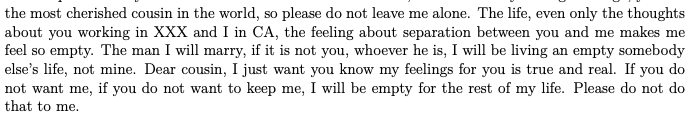
\includegraphics[width=.9\linewidth]{./pic/backups_plans_20210423_201706.png}
\end{center}

而且我心中对我表哥的认定(或者说是爱情信仰)是:如果我结婚、如果我嫁的人不是我表哥,那我再嫁给这个世界上任何其它人,我过的都终将是其它人的生活,不是我自己的,我做不成自己、成为不了我想要成为的人,我都将无法幸福!(对我表哥的这份认定,始于那场告别,但对这份这定的表达,所有传记文档里最原始的纪录是3、22、2012写给我表哥的邮件里。)

这里,我有一个很大的疑问:

\textbf{为什么想要结婚了,我却没有去找表哥,为什么当年的我像是把我亲爱的表哥给弄丢了?还是,当年的自己,为什么就自己走丢了?}

\begin{center}

\includegraphics[width=.9\linewidth]{./pic/backups_plans_20210426_112108.png}
\end{center}

\begin{center}

\includegraphics[width=.9\linewidth]{./pic/backups_plans_20210426_114722.png}
\end{center}

\begin{center}

\includegraphics[width=.9\linewidth]{./pic/backups_plans_20210426_114834.png}
\end{center}

这些个,一系列的,前后共分五次——或被动或主动、站出来写的《成长的故事——我和表哥》系列,任何时候我站出来写,我都是按照传记作者、记载者我自己当年当时情境下的真实想法来记载的。

那么我们回来试着寻找一下当年的境况。

\subsection{(三)当年我把自己走丢了}
\label{sec:org6df2c38}

我们来理清楚我这次——第五次地站出来写的前因后果是了什么,是如第二次收到我表哥的邮件、我所感受到的那样社会大众无法理解我表哥与我超越世俗的爱情,所以我必须主动站出来写出自己的家族亲情爱情故事来给我这一方的当事人提供社会大众理解的视角与机会?

不是。当时是我对舅舅的理解、对我亲爱的表哥与我这份爱情的理解与事实有着很大的出入,当受到三大舆论洗劫影响多年,当近几年的自己内心里有个声音一直在呼唤:为什么我亲爱的表哥就是不喜欢我,为什么我亲爱的表哥当年就是说十年之内不会结婚?为什么我的舅舅就会如三大中文舆论所指出的那样错换人生,将我原本美好的后半生换成了舅舅的亲侄女大表姐在硅谷的后半生?

我不理解,我心中有恨,我对舅舅的恨无法排潜,当这所有的一切我都理解不了、苦苦思索却找不到答案的时候,我找出了自从自己写完了一遍、2015年最后一次整理一遍便再也不曾回去读过的、自己分几次多次站出来写的自己的传记时,3、13、14的这个周末我回去看读了那些传记,重新回味了那些年月里的自己,多么幼稚、多么自卑——尤其是2012年秋天回去重读《计算机专业》之前!

虽然距离少小时候的自卑已经过去很多年,但它并不会简单完全褪去。那些年月里自卑的自己、也伴随着一定程度上的感受周遭事物认知上的缺陷,即便是在我喜欢得不得了的我表哥与我的相处过程中,有些情节、有些场景或许当时那颗自卑的脑袋扫描到过,但却也仅只存在于脑海里,而没有经过任何的思索与加工,没有为我带来他们应该给予传达给我的信息与信心。

最显著的,举个例了吧。

\begin{center}

\includegraphics[width=.9\linewidth]{./pic/backups_plans_20210426_161140.png}
\end{center}

2011年11月的记载中,关于2010年8月头我怒气冲冲杀回去找舅舅报仇时,关于我敲我表哥房间门的纪录如上。 

\begin{center}

\includegraphics[width=.9\linewidth]{./pic/backups_plans_20210426_161859.png}
\end{center}

\begin{center}

\includegraphics[width=.9\linewidth]{./pic/backups_plans_20210426_161924.png}
\end{center}

但是当今年三月中旬,我再回去读,这又过了十年、显然已经比较成熟自信的自己,便最终能够想起——并消化掉深藏在脑海深处,但不曾加工处理的关于我表哥房间门的这层意思。

当我有了这些想清楚了之后的信息,我便有了坚定的信念:表哥是喜欢我的,我表哥他从来都是喜欢我的,只是我自己自卑、不曾真正接收到这条肯定信息、对我表哥缺少了应有的自信与信心!

\begin{center}

\includegraphics[width=.9\linewidth]{./pic/backups_plans_20210426_162149.png}
\end{center}

所以那天今年三月,写到那里,这次回来再写、重写、接着写与梳理好我亲爱的表哥与我的爱情,我便开始用自己的文字来表达同我亲爱的表哥之间的精神恋爱了!

\begin{center}

\includegraphics[width=.9\linewidth]{./pic/backups_plans_20210426_162643.png}
\end{center}

但那些年月里幼稚的自己、与如此强大又待自己特别好的我表哥面前,我尤其的自卑、自卑到如果感受不到表哥对我的喜欢,我就跑出去玩,去加州找朋友玩儿,不回来!而对于表哥已经表达得很清楚的意思,我一方面感受环境能力有限、另一方面消化理解有限(源于当时自己自卑的心态?),所以表哥原本可以传达给我的很多信息都被我华丽丽地忽视掉了。

\begin{center}

\includegraphics[width=.9\linewidth]{./pic/backups_plans_20210426_163310.png}
\end{center}

\begin{center}

\includegraphics[width=.9\linewidth]{./pic/backups_plans_20210426_163417.png}
\end{center}

那就导致了一种心理局面:

\textbf{我表哥明明是喜欢我的,我却不知道(在我表哥对我的喜欢上始终都表现出一种相对脆弱得多的信心——如果有的话,较之于自己喜欢我表哥,我对他的100\%肯定与认定来说)、信心不足;}

\textbf{但是我知道我一定是喜欢我表哥的!更知道,我表哥曾经为了我保持他原本的身材接近一年半的时间;我知道表哥为了我的一句问话,曾经真真切切地努力锻炼、把他锻炼成无数少女心目中如痴如醉的梦想过!}

\textbf{我亲爱的表哥为我真真切切地付出过、用行动的!不是像我用嘴巴说的用耳朵听的。}

而这,便成为毕业去到加州后支撑我战胜所有三大舆论制造险境、艰难险阻而绝不掉进去的原因:

\textbf{我亲爱的表哥,曾经给予过我这个世界上最美好的爱情!为了自己心目中对我表哥的这份认定,我也绝不允许自己沉沦、陨落,哪怕是我走着一场快餐速食般将就着的婚姻!}

\begin{center}

\includegraphics[width=.9\linewidth]{./pic/backups_plans_20210426_165635.png}
\end{center}

\textbf{如果真是因为那时自己的行为幼稚导致我表哥不够喜欢我,那我守好自己、只要表哥还没有结婚、只要我守好自己,留得青山在,不怕没柴烧,总有一天,我亲爱的表哥与我,还是有机会能够走到一起的!} 这是后话。

\begin{center}

\includegraphics[width=.9\linewidth]{./pic/backups_plans_20210426_163905.png}
\end{center}

而我,在表哥希望我也能够稍微瘦一点儿、自己说过自己太胖了的时候从来不曾为表哥做出过任何的改变。这是对我表哥的一种永远的亏欠——仿佛我从来不曾对我表哥付出过真心一般!

\begin{center}

\includegraphics[width=.9\linewidth]{./pic/backups_plans_20210426_164137.png}
\end{center}

而到后来,与12年4月与舅舅见面的聊天里、以及后来我作决定留在这边不回去时,我完全就变成了一个因为舍不得我表哥而坐在地上发奈的孩子般:因为我表哥曾经给予过我的好,我绝不放手!留得青山在,不怕没柴烧!我就要留在这里!

\begin{center}

\includegraphics[width=.9\linewidth]{./pic/backups_plans_20210426_113411.png}
\end{center}

\begin{center}

\includegraphics[width=.9\linewidth]{./pic/backups_plans_20210426_113704.png}
\end{center}

可是一年后经历了昨时隔离令(自3、7、2013隔离至3、7、2014)、经历了暑假实习对自己小导师A的工作相关的近距离观察欣赏与接触,我的灵魂仿佛在游走!(记录于2014年夏天SJSU的楼书馆)。

我想,我那时想要游走是一种心态,是一种对我表哥对我爱情的态度不敢终极肯定、自己也想要出去玩耍、想要流浪的一种状态。

\begin{center}

\includegraphics[width=.9\linewidth]{./pic/backups_plans_20210422_075555.png}
\end{center}

同自己心目中父爱如山的父亲相比,我表哥在我这里似乎缺少了某些精神力量:那在当时的自己,我亲爱的表哥、无比亲切的表哥,就只能算是一个曾经的陪我玩耍过的大伙伴而已了?!!!

像那个四岁坐在牛背上的孩童,我知道我表哥喜欢我,可是我想要出去玩耍、想要出去走走,却一不小心、玩兴大发,把自己走丢了?!!!一方面我表哥给予我的爱情他不曾语言肯定过,而我有一颗流浪的心,我还没能完全割舍对大城市的眷恋,可能这也是一个原因。

\begin{center}

\includegraphics[width=.9\linewidth]{./pic/backups_plans_20210422_075830.png}
\end{center}

那时2014年夏天作自传纪录的自己不明白、接下来的2015、2016年自己、乃至于短暂性失明一头撞进尘世婚姻的自己仍然不明白:

\textbf{我那深深爱恋、掩藏心底的我亲爱的表哥与我,在我这里所缺少的只是时间的沉淀,只是《用来检验我表哥与我是否真爱的》外力作用来帮助我认知我表哥在我这里《确实存在、始终存在的、但是自己并不知晓》的精神力量而已!}

\textbf{但真正认知、深切感受到这股外力、经受住这股外力的严峻考验、并最终认识、找回自己却已然贯穿跨越过了那场尘世婚姻!}

\subsection{(四)当年选择了安于现实:走进世俗婚姻}
\label{sec:org5c5d144}

当时从学校回到加州时的自己的状态,现在回想起来都不知道该如何形容。当年的自己应该是说过五年之内、十年之内都不会回来之类的话吧!

那时的自己,我没有任何回头的心境、也无法回望我亲爱的表哥与我那惊心动魂的爱情。 

而现实生活面前,我还有自己高龄生育的压力,而我本身身体又不好。

\begin{center}

\includegraphics[width=.9\linewidth]{./pic/backups_plans_20210424_095212.png}
\end{center}

\begin{center}

\includegraphics[width=.9\linewidth]{./pic/backups_plans_20210424_095046.png}
\end{center}

当我走进死胡同、两眼一抹黑,我就走到了自己曾经感慨过的那“或许有一天,也我不得不走”的广大小市民常走的路:我抓住了一根救命稻草,走进了一场现实中将就着过的尘世婚姻。

现实中,就像是抓住一根救命稻草一般将就着的婚姻,大可不必言谈感情,能将就着把日子过团圆,已然是很大的奢望。

然而即使如此,在真正的将就而成的婚姻里,仍是奢望而不得圆满。这是后话。

\begin{center}

\includegraphics[width=.9\linewidth]{./pic/backups_plans_20210423_204215.png}
\end{center}

\begin{center}

\includegraphics[width=.9\linewidth]{./pic/backups_plans_20210423_204134.png}
\end{center}

那时的我因为连续一年多的时间都还在硅谷学校里读书,应该是还不曾看清三大的本质,受当年成名与房东的朋友相亲的影响,我也走了她曾经的老路,虽然是在自己又回到学校读过三年的《计算机》拿到了硕士学位之后。

\begin{center}

\includegraphics[width=.9\linewidth]{./pic/backups_plans_20210423_202941.png}
\end{center}

2010年5月我在加州第一次租房间住,他——我后来尘世中将就过的婚姻中的对象,与我共同一个房东,他已经在那里住了很多年了。 

那时刚搬到那里去住的我,对那片地方周围的环境也不熟,一次打招呼聊天聊起,他也曾帮忙带我去过家旁边的walmart。

2012年我返校后,他13年曾帮忙把2012年春天在Paypal工作过的我的2012年度税表(还是2013年帮我寄过2012年的税表)寄至我在外州的学校。

2016年夏秋(那一年从元月起我就租住房间,离我原房东、离他也都还比较近),家旁边的99大华超市里,我碰见了几年不曾见面的他。稍稍聊了几句,他问我可有他的电话号码?我说是的。

\begin{center}

\includegraphics[width=.9\linewidth]{./pic/backups_plans_20210423_203401.png}
\end{center}

感情里、婚姻的归宿上,我一直以为自己从来都是有着闪婚情节的,就像当年与我亲爱的表哥,相处了几天,我便说服了家里所有的人,俨然一副那姑娘马上就要出嫁了的样子。

但那学校里连续上完三个学期后,第四个学期是可以休学(前三个学期共交了\$18000的学费)不用交学费的。我考虑了这接近四个月的时间,眼见马上就又要交一个\$6000的学费了(,在交了昂贵的一万八之后,我手上连交学费的钱都不够),最终决定把他约出来聊一聊,探求一下双方的意思。

约在一个公园。我向他讲述了自己的学习、工作生活中过往与经历。他也讲了与他相关的。 

来自于越南难民。但却仍然是那个年月、他们那个年代里绞绞者的存在。比我大23岁,比我亲爱的表哥还要大出10岁,应该还是会比较懂得照顾人吧!

如同自己的三姐初中没毕业就踏入社会了,如同自己的二姐中专毕业也早早地踏入社会了,如同自己的大姐高一没上完就踏入社会了,他踏入社会也很早,靠做塑料购物袋挣钱,先攒购钱财帮助把两个相对年幼的弟弟、走黑路偷渡将他们先送出来,然后他才再攒够钱自己跑了出来。

他应该是如我现在这种境况般社会底层的平民老百姓,又不同于我常年生活在校园、生活了大半辈子,他因为踏足社会很早(可能就相对于初中的年龄就入社会了),对这个现实社会有着根深蒂固的世俗观念与偏见。他生活在俗世,我却如同我亲爱的表哥属走心派,生活在灵魂深处生活在“灵界”。回想自己长大后与三个亲姐姐的隔阂,基本只与父母最亲更亲,我会受得了他的世俗吗?但我也不曾多想深想。 

\begin{center}

\includegraphics[width=.9\linewidth]{./pic/backups_plans_20210423_211802.png}
\end{center}

也还算是拥有亲情吧。

\begin{center}

\includegraphics[width=.9\linewidth]{./pic/backups_plans_20210423_213157.png}
\end{center}

得不到想要的我表哥的爱情的我,与自己那领养来的叔叔家的大堂妹一样,尘世里好歹还算是遇上了一个同自己一样拥有亲情的人,我以为我们能够把我这尘世里将就的婚姻过团圆。

\subsection{(五)那年我结婚了}
\label{sec:orgd9b4505}

去赌城登记注册结婚前,我病倒了,除了2001年夏天7月29日必须做手术医治之外平生最严重的一次平民百姓百家病:连续几天发温高烧,晚上睡前会咳大半夜,去往赌城的路上,嗓子咳破了、耳朵一路鸣叫!在赌城的一两天也一直不见好,我——快死了吗?

\begin{center}

\includegraphics[width=.9\linewidth]{./pic/backups_plans_20210423_213744.png}
\end{center}

2017年1月6日,重病中的我与他轮流开车前往Las vegas,晚间抵达并密秘登记结婚了。虽然四年后,我还是去办离婚了。

说是密秘登记,是因为当时极端环境下的自己,已然没有胆敢、没有敢要光明正大开车前去赌城结婚的胆量。甚至于,先前与他的联系、见面都丢开了自己的手机、私下密秘进行。

\begin{center}

\includegraphics[width=.9\linewidth]{./pic/backups_plans_20210427_120126.png}
\end{center}

不是说,不能够与自己心底深爱着的表哥结婚,而去将就一份尘世里的婚姻就有多么可耻,而是过往三年我所选择的神等级的《计算机》专业学习过程中被野鸡大学院第里一直搞孤立、一个院系、一所学校动用所有师生、同学、以及打工所在的学生食堂、动用一切他们可以动用的力量来针对一个小小国际留学生进行打击勒索、这种动用所有力量来针对一个个体的暴力行径,才是最可耻的!

但那场暴力的受害个体——我亲爱的表哥曾对我倍加宠爱的这个小弱弱个体,想要从那场风暴中走出,显然不是表姐简单带我去海边玩儿一次就可以平复得了的。

又经历过一个2016年的四月1日,又一次申请H1B工作签证的机会,又一次地没有任何收获!2014、2015、2016,多少次地向往过,便有多少次地失望与绝望!

我对这个社会的认知、这个学生学习、工作、工作签证体系的认识到底还停留在什么层面呢?

我向往过、失望过、绝望过,一次次地撞向南墙,又一次次地碰壁头破血流,一次次地扑灭了梦想,生活中的困境一再打磨着我:学会沉默、学会规避,像鸵鸟一样把头扎进砂子里,像乌龟一样把头脖子和四肢都缩进去!

我现在已然是这个社会最底层的最普通的平民老百姓,我还有什么可以争强好胜的?还有什么事是我可以出头的吗?还有什么是我出头就可以有所收获和拥有的吗?

我退缩、我畏缩,我把自己躲起来、藏起来,把自己躲藏到自己感觉安全的地方。

比如,这场自己一开始就清楚地明白:这是一场将就的婚姻。但在生活的恐惧里,哪怕是将就的婚姻,你又如何能够保证:你想要将就、想要去结的这场不顺从内心的婚,你就一定结得成呢?

想当初,我对家里所有亲人的思想工作都做好了,俨然一逼这姑娘就要出嫁了的样子,可是我想结的婚呢?婚没结成,不是还是被舅舅打了911、被我亲爱的表哥打了911吗?

当我选择了《计算机》这个神等级的专业回去读书,我的回报又是什么呢?不是照样被野鸡大学、被那个神等级专业的院系痛打落水狗般暴力施暴?那份伤害,又岂是普通如你我般脆弱的灵魂就能简单轻易承受得了的?!!!

我——没有理由不去躲藏!一场婚姻,只有那张结婚证拿到手、获得它应有的法律效力,那这场婚才算是真正结了。其它所有的一切,都是浮云。

真正登记结婚后,平安归来回到加州后的我,打电话给大姐夫,告诉家里所有的亲人,我已经结婚了。姐夫略有不悦、不够放心地问我,为什么我结婚前就不曾告知家里任何人、就那么草率地把婚给结了?婚姻大事,我怎么就处理得这么轻率、草率!!!

我惊倒,懂得自己的莫若家人亲人。想我不是走投无路、万般无奈、抓住一根救命稻草,谁愿意去将就这尘世里妄谈感情的婚姻!

可那场轻率、草率将就的婚姻苦果终究还是得自己去品尝。

结婚后,不再是像先前人生没有着落、甚至不知道是否最终会像大表姐曾要求我的那样、最终不得已在这里黑下身份来,我觉得自己遇见了光明,我把这个尘世里将就的婚姻、我结婚了的消息告知了大表姐。

2015年大表姐的工作:饭桌上大表姐把她的手机拿出来,翻出来里面的照片给我的看她在2014年夏天我写完《成长的故——我和舅舅》第三次详细记载两年《计算机》专业学习之后,她的工作单位三星帮她安排了一次秋冬季出差时所租住房间的照片。

大表姐说,她是组里的核心灵魂人物,少了她很多项目是无法运转的。而那次单位给她安排的出差,同样是去西雅图Microsoft去解决一个什么问题。陪同她一起前往的,还有当时大表姐site里另一个相对年轻得多的男技术总监。大表姐说,可能当时安排出差的时候,单位也是有点儿担心,怕她搞不定这样一个项目,所以技术总监也跟随着。后来她确实有绝对的信心能够解决问题之后,技术总监才先行一步离开,而大表姐当晚解决问题后已经很晚,便在当地住宾馆休息。

\begin{center}

\includegraphics[width=.9\linewidth]{./pic/backups_plans_20210427_184530.png}
\end{center}

世俗聪明如大表姐,当然也清楚地知道,这是单位给她一次拔苗助长的机会——彰显她在公司的重要性(即便她有可能实际上并没有那样的实力或地位),便当然会世俗聪明地租住了主街上那家宾馆最豪华的套间,超出了公司正常可以报销的预算。但为了打出她的知名度,谁会真的在乎超出的那点儿预算呢,就算是她自己掏腰包出1000块钱,那种情况让她扬名立万树立战功的境况俗世聪明如她、她会犹豫吗?

这一年,自2006年我来到美国,大表姐便也分头从加拿大来到硅谷谋生存以来,9年过去了,2015年与我见面,大表姐说,公司很好,公司终于帮助她申办了工作绿卡,她以44岁高龄、(没有本科学位,不曾考任何英语语言考试)硕士学位、完全没有任何工作经验的白手打天下,终于于这一年在这个国度获得了一席生存之地!!!

大表姐再与我聊她的儿子远在加拿大贺笨笨的事。大表姐说为了把他给弄过来(弄到美国来),没有别人的办法,只能先把他哄过来(美国这边)玩儿,让他坐海船去海上钓鱼。他来了让他作主选买张一辆豪车,希望能让他动心,争取给他树立一点儿向往、把他也给想个办法弄过来。 

2015年夏天那次在Montery的海边上,大表姐带我在大岩石上躺下来晒太阳。大表姐说平时太忙了,现在能够这么躺在岩石上晒太阳,好舒服呀。

我们都找块石头躺下来,大表姐与我聊天说,人都活到这么大岁数了,什么事儿都该看透想开了,还没有看清楚爱情算是怎么回事么?再惊天动地的爱情到头来还不是柴米油盐酱醋茶?!这到个岁数、结不结婚有什么关系?!生不生小孩有什么关系?!以后就该怎么开心怎么活!

大表姐的话我听得非常刺耳、很讶异!但大表姐的话在我当时就是过耳东风,就是当时的海风,吹过了就没有了。而我心心恋恋的我亲爱的表哥,不知道什么时候才有机会可以再走到一起呢?

2016年1月我出来自己租房间住。1月9日,大表姐去给小表姐的孩子加根线,顺便帮我也加了根线,每多加一根,月租贵\$20,一次性激活费也是20块。 

17年我结婚后,把结婚的消息告诉了大表姐,表姐说我们出去吃饭。她说Sunnyvale哪家西贡好,约到那里去吃中饭。于是我与他先去排队,等她来了三人一起吃了一餐。

表姐送了件小毯子,买一把花。当时三个人吃了六七十块,我把一年来表姐给我出电话费的\$500拿还、预付给了她。

那次吃饭回来,三大舆论说大表姐、我们三个人吃得、花得太多了,但不久大概几个月后我与自己当年小伙伴板块的两个人的一餐饭吃掉了一百多块却听不见三大报怨任何?!!!

关于野鸡大学校友、系友板块、与男闺密的其它事情打算开个专题,把与我一起,三个转专业的放在一声儿来写,这里暂且不表。 

17年再联系上表姐,就知道她买了新家,去表姐家里也看过。表姐也再次与我讲述了、像是借我之耳表达她的感激般,讲述了她的儿子贺笨笨的电梯经历。

那是13年夏天我当时实习时组里的喜欢talk talk style的项目组长C于15年又调到了苹果去工作了几个月。而当时笨笨的比较优秀的同学们已经有几个直接被招进了美国这边的苹果,但笨笨没能通过面试没能过来。笨笨那边关于他同学的消息应该也是第一时间反馈给了大表姐。所以当经历了2013年那个夏天特殊时期、特殊组队的、后又解散队伍,并与C保持了经常联系的表姐听说C在苹果工作后,便请她帮助把笨笨的简历递交给有需要的任何组,便就有了接下来贺笨笨电梯直进苹果的结果。笨笨进到苹果后不久,C便不知什么原因离开了苹果,像是在哪里(不管是先前在三星,还是后来在苹果)都是在打游击战一样。 

\subsection{(六)那年我怀孕了}
\label{sec:orga8daa03}

我们一月份结了婚,但当时还是分开住着,到二月份才找到房子,搬去了sunnyvale一个apartment住一个在客厅改装成的大房间,带个小阳台,\$900每月。

两个都单身很久的人,最开始的磨合、相互认识是很困难的。

我喜欢吃海鲜,我们买过一两只螃蟹回来吃。他说要青岛啤酒一起吃才好吃,于是我们买了一瓶。

他说他不喜欢吃螃蟹,而我,从来都是爱极了鱼类爱极了海鲜的,于是,我就把剩下的吃光了。

改天我们买了一个西瓜。前一天刚吃了一点儿,第二天我再打开冰霜,没有了!我问他,他说他以为我不喜欢吃西瓜,所以他把它吃光了!

然后我才告诉他西瓜太甜了,不能一次吃太多,要慢慢吃每天吃一点儿才好。

如我般,他也是一个资深吃货。他总是说,什么什么东西放久了就要放坏了,需要赶快吃,然后他自己找自己、默默地背着我把它们吃完。我也不多话。

如果一座婚姻里,他想要吃的东西他都吃不到吃不好的话,那就太没什么意思了,至少同处在这座婚姻里的我,做不到。

于是我放任他吃,想吃什么,只要不是太离谱,都顺着他。

那个时候,COSTCO的大力菠菜——大大袋大概是2.5磅卖4.5美元,里面全是小菠菜叶,不像超市里卖的中国菠菜,不是一棵一棵,全是叶片顶端的菜叶、基本没有梗的,他很喜欢。

遥记得2012年到2013年秋季学期,那时还在学校食堂里打工的自己,常常拿沙拉吧的这种菠菜叶和蘑菇吃,被三大用来培养共情、打趣儿起梗、造了个好玩儿的梗儿发网文说,《大力水手吃了菠菜会变强大——是真的!!!》于是,每每到了超市到了costco,我总是打趣他说,“大力水手想不想吃菠菜了呀?”这个大力水手吃菠菜的梗儿被我们玩儿了很久。

但他似乎并不感恩于我待他吃东西的好。等我想要吃什么东西的时候,他总是阻拦。如果一座婚姻里,注定有一个人吃东西吃不好的话,那与他的这一座,我便是那个吃不到、总吃不好的人,但我还是得让着他,这一点儿我对他从来都问心无愧!

久了就发现,除了红尘男女每天都需要的吃饭之外,我们竟是找不到任何可以聊天的话题。

那时的三大天天吹风,天天说什么谁谁谁假结婚。可我是选择了与他过世俗日子的。

记得那天去赌城登记结婚登记的当晚,我们找一个租住的地方,前台说多出十块钱可以住一个加了一张床、有两张床的房间,我病得昏昏乎乎不明所以,他同前台说加十块钱租了有两张床的房间。但我还是选择了躺在同一张床上,当时我已经病得很严重很累了,我躺上去就基本睡着了。

或许那时三大的风,我还并没有能够分辨清楚是真刮还是假刮。但在那个极力隐藏、极力躲藏自己、恐惧不安的岁月里,倍感恐惧的心总还是会找到解脱办法的。

半年后,38年前半段人生中,我第一次怀孕了、很意外。我很慌乱,不知道接下来该怎么办,我跑去COSTCO买了瓶补叶酸的保健品,可是我开心不起来。

是的,我想生孩子,体会一次做妈妈孕育生命的幸福,但我想生的是我表哥的孩子,不是他的!!!

半年里,我们建立起来什么呢?

与其问建立起来了什么,不如问我们失去了什么,为哪些事情争吵过、动手过?

我以为我的脾气很暴躁,把我惹毛了我会很恼火的;但见识了他的火爆脾气之后,我甘拜下风!

\begin{center}

\includegraphics[width=.9\linewidth]{./pic/backups_plans_20210427_195919.png}
\end{center}

舅母问我的时候,我还申明说,要是把我惹火了,我的脾气可大着呢!

那是我还没有见识过他的脾气。

一个大男人,一句话不对口,整个人就青筋暴出、变得暴烈起来、咬牙切齿、眼睛瞪得像恶狼一样,整个人残不忍睹,他却还要动手打人,不分轻重,不知道他是个男的,手很重,凡他下手过的地方,身上总会轻一块紫一块儿的。

我的记性不是很好,打过多次我也都不记得了,就像我现在去回想2012-2015三年里神等级的专业里很多发生过的事,我只就住了相关的一些点,大部分的事情联系全被我忘光了,除了读自己的传记尚能够忆起的部分。

我只记住了他每每凶狠恶刹的样子,在家被打过很多次,在与他同去的赌场里也被他揪胳膊手臂揪出很多青紫,鬼腾赌场的工作人员也曾当面警告过他。

在我这里,他有句名言,就是所有的错都是我一个人的错,都怪我,要不是被我激怒,他才不至于不会想要去打人呢!

他却永远认识不到,这个世界上没有任何人想要激怒他,他所谓的被激怒,也不过是他期待太多、心里或有太多不平、他苛求得太多!

我不想说他不容易与别人想处,因为他与他同事等社会关系他处得还算是很不错了。

那么,为什么婚姻里,他就会有那么多的怒火、想要索求无度呢?

在我之前,他结过婚,又离了,维持过五年的婚姻,但据他后来讲起,他与其前妻更像是假结婚般,只有很短的一段时间住在一起,后来就分开住了,直到最终离婚两人彻底分开。说起来,那也是他与我结婚十年之前的事儿了。

我问起过,他说,他前妻就常常给他做好吃的呀,一如当初我们约见面在那个公园时,他会反复问及我素日里都吃些什么、是否饮食习惯少油少盐、是否饮食习惯健康等。

可是我总是做好吃的给他吃,他却牙齿很长、从来不知足,并不放在眼里。

而我总是让着他吃,他却从来都假装不知道是我在让着他,尤其是吃各种肉。

我虽然是吃菜吃鱼长大的孩子,不爱吃肉,总是用一点儿肉调个味道就可以了,但这并不是说我任何时候都不喜欢吃肉、或任何时候都只能吃很少的肉,我想吃的时候,他极少满足我,而有肉的日子,肉都拿去给他吃了。 


三大对我是实时监听的。当得知他们的被盯当事人怀孕,他们可能并不如我般意外,但他们也是慌乱的,他们在网上炒作说,一个女人生了孩子,就会从此被拖累,一个女人自己带孩子是一件很痛苦的事,并且生一胎傻三年,以后工作事业上再没有任何发展机会之类的洗劫。

三大舆论炒作说,当有一份工作与一个孕育中的生命摆在面前让你选择的时候,你就应该选择工作!

三大那一次的炒作洗劫是合乎我心的、深得我心,因为我没有准备好,与他租住在这样一个破烂环境中的我们没有任何一个人准备好,我以为、认为他和我一样拥有亲情而结婚,但他的亲情只向他的亲人(他的亲兄弟姐妹)表达,他的意外灾害保险受益人从来都是写的他远在纽约的弟弟或是哥哥的名字;而我既不是他的亲人,也不被他当作爱人对待。我们没有任何理由要脑袋锈逗了、冒这么个险去生一个没有准备好、不被欢迎不被接纳来到这个世界上的孩子。 

于是,他们三大发动舆论,在他们一波一波舆论的炒作洗劫里,在我与他一次次地争吵里,换来了三大为迫使他们的被盯当事人不会把孩子生下来、而用作交换的紧急事件紧急处理的、快速locate被盯、将来被职场被逼当事人到他们的客户端——我在local Sunnyvale的一份专业相关的工作——头衔是安卓开发工程师。

后来,再经历18年我辞职后职场生涯被彻底封死后我转向非专业职场生涯谋生,经受他们再一波对非专业职场女性逼良为娼的舆论攻击与操作后,我终于明白,这时三大 \textbf{一定会} 用一份职场工作来替换掉他们的被盯、将来被逼当事人生育的机会。因为如果一个女人一旦生了孩子,那他们三大中文那么多年来紧盯、看守的女色资源的利用、或转手价值(如现在将其locate到他们的职场女性性奴合作小公司他们的客户手上所能获取的黑色利润)都必将大打折扣,这是他们不愿意损失掉的!

尽管他们原本极有可能还打算再拖一段一时间、让当事人再坐冷板凳久一点儿、再拖一拖被盯当事人的电梯投放时间,拖的过程中试图想要与被盯当事人再炒作炒作、共情共情、磨合磨合——磨合出他们想要的你情我愿、半推半就、互惠互利、友好共处的职场合作未来?!!!

这些,是我后来经历过非专业相关职场再受遭受到三在舆论的逼迫与攻击后体悟出来他们的逼良为娼的本意。 

咦,怎么这份我意外怀孕、情急之下被三大紧急处理、用一份工作换来我人工流产舍弃一个没有准备好来到这个世界上的生命时,三大继2011.2012季两次电梯投放之后,这次我因为拿到结婚后工卡接下来就可以合法工作的第一份工作,他们一推就把我就推到了就在我们所住的local、就在离Sunnyvale我所租住的地方不远呢?

回忆一下,这简直与一年多前我野鸡大学的校友、系友板块同学2016年找工作时被——“野鸡大学的院系里”一推,他便被推送到了他所居住地Sunnyvale local家旁边的AMD如出一辙。

\begin{center}

\includegraphics[width=.9\linewidth]{./pic/backups_plans_20210413_131623.png}
\end{center}

\begin{center}

\includegraphics[width=.9\linewidth]{./pic/backups_plans_20210428_094132.png}
\end{center}

历史惊人的相似,每天都在上演——那句久远的“性格决定命运”呀,冥冥之中自有天意,是耶非耶???

天意是什么,天意是神奇的预见能力,能够未卜先知地将这们这此即将工作的待业“青年”随即推到他们家旁边的某个公司?

天意也是后来2018、2019、2020年里当三大舆论天天炒作说表姐在美国得以立足、安闲度日的后半生是我的舅舅发动三大舆论错换人生——是把原本属于我的美好的后半生换给了我舅舅的亲侄女大表姐的时候,幼稚的脑袋苦苦追问、灵魂拷问:我亲爱的舅舅,为什么会像三大舆论所炒作、所指出的那样“利用”我,将我原本美好的后半生借助三大舆论之力交错替换给了他的亲侄女大表姐时,天公所给予我的回应\textasciitilde{}!!!

国内娱乐圈前几年无所不用其极地曾炒作出过一个“雨神”萧敬腾,据说是只要他一开演唱会一开任何商演活动,老天就一定会下雨!!!

\begin{center}

\includegraphics[width=.9\linewidth]{./pic/backups_plans_20210428_095419.png}
\end{center}

而与他婚后后来岁月中,我心目中也慢慢有了自己生活经验中搭建树立起来的“雨神”(那人类灵魂的工程师之前的称谓),那就是——我的舅舅。

我头上有畸角、我身后有尾巴,我是一条小青龙、小青龙、小青龙。。。。。。儿歌里是如此唱的,这只少女心小弱弱常常也会钻进自己思想的畸角里,当时的自己竟怎么也走——不——出——来!!!

每当我思想有死角、每当我对我亲爱的表哥所给予过我的爱情信心不足倍加怀疑的时候,每当我回想、追忆起来理不清头绪、对我亲爱的舅舅心有怨念、心怀仇恨,每当我只要在微信上一发朋友圈、发关于我想不通的关于我亲爱的舅舅的我的思想死角,就一定、一定、一定会迎来加州硅谷南湾的变天——骤变天气:电闪雷鸣、天降暴雨、六月飞雪、三月冰雹!

去年还是前年的时候,因着对舅舅的不理解,加州硅谷南湾酷暑天气的那个我发微信朋友圈的晚上雷电交加、响彻天际、电闪雷鸣后天降暴雨,让躺在床上的自己惊诧不已,也反复摧残、蹂躏着那颗灵魂发问的心:我做对了吗?我是真的错了么?!

去年六月,我的微信朋友圈一出,老天爷的脾气之大,更是六月飞霜!我们《语文》课文学过《窦娥冤》,难道我亲爱的舅舅,被我一再发微信朋友圈灵魂拷问的我亲爱的舅舅,就真的是如这六月飞霜般——有冤无路诉、以致天公老天爷要亲自站出来昭告天下、表达对我的愤焖?!!!

\begin{center}

\includegraphics[width=.9\linewidth]{./pic/backups_plans_20210423_230138.png}
\end{center}

那时,我亲爱的舅舅,被我这个远亲的侄女冤屈得,简直就是世界之大悲剧,亦无愧色也!

今年三月,当我实在想不通、敢冒天下之大不玮、一再苦苦追问,为什么我的舅舅会做出如三大所传递给我的、错换人生那么背叛自己的事情时,更是天降冰雹?!!!

\begin{center}

\includegraphics[width=.9\linewidth]{./pic/backups_plans_20210422_090142.png}
\end{center}

我一直口口声声念叨着的,我幼小的内心、稚弱的灵魂自小便崇拜、景仰着的:人在做、天在看、天地良心的、我隐藏心底、一直秉承着的、一直景仰的大自然之神——老天爷呀!

难道我就真的错了吗?

为什么我只要一出声,你就会如此骤变、发脾气来回应我、怼我?我一直景仰、支撑着这个野草般顽强疯长的小弱弱我的天地至公的老天爷?!!!

上面这些,是那个被我亲爱的表哥万般宠爱过的我表哥眼中的少女心小弱弱,当年把自己给走丢了之后很多年后来年月里的心事。 

后来,在我苦苦追问找不到答案的时候,在我终于找出自己的传记故事、读出当年自己的自卑与幼稚、找回自已的爱情后,这些疑问也便风飘云散了。这是任何读者都应该数数脚趾头就能够明白的逻辑。也算是后话吧。 

又或者,当年,“我们”租住房子的时候,“冥冥之中自有的天意”(三大中文媒体、舆论)便早已插手、着手安排、布置道具着如我般“棋子”托儿们、小弱弱的人生?

2009年秋季我《统计》专业的最后一个学期,我有选一门计算机专业CS120编程的课。后来我实习的29个月里,板块与男闺密是如何转专业去读计算机专业我并不是很清楚,只知道他们两个同专业的系支或是同班同学关系还挺好的。我12年秋天回去读书,他们两个大概是13年12月两人同时毕业,校园内呆了一年,14年12月底两天一起开车前往加州硅谷,准备找工作。 

当时我也是有在三大中文上看见有人发贴子说他有一处好房子,车库改装的两个房间,租金便宜,不希望好房间落入“外人”手,所以特来他们的网站发贴,希望能够租给“品行良好的同专业”的小伙伴们。并还声情带冒般地说,希望版主体谅,不要删他的贴子。 

这些只是意会。当年闺密与板块是如何找到一处车库改装的两个房间,两小伙伴还是同住一处的过程我并不是很清楚。

但是后来同闺密与板块的相处,15年我申请加州硅谷挂靠学校需要提供国内成绩单的校对证明,闺密开车与板块陪我前往UC Davis办证明,15、16年的我常常俗世里打工打着打着就把正在打工做的一两份事儿给打没了的时候、16年板块被公司按排回国工作一年——应该是希望借他在国内工作一年的机会能够解决个人婚姻问题吧,回国前与回国后板块说过的话、做过的事、板块从中国上海回来后,三大狂刮过一阵儿扫荡的风专门为板块洗地、帮他解释他在上海一年没能如愿解决其个人婚姻问题的原因等——都一再告诉自己:这是自己小伙伴队伍里隐藏得、埋藏最深的从一开始便投奔了三大黑势力、作着三大的托儿的迷惑等份内工作存在的时候,我便终于明白:野鸡学校育人无方,教出的三个臭皮匠(闺密、板块和我,三个转专业的计算机神等级专业毕业生)还没有一个能好好地找到工作,当时当他们两个人的OPT只剩下最后一次申请H1B工作签证的机会,当三大舆论的风狂刮过野鸡大学的校园,校园里院系里大牛等LinkedIn里强推板块出来工作(以示野鸡大学还是出人才的,野鸡大学的转专业硕士毕业生也还是能够找到工作的!),便有了板块被这么一推就推到了家旁边AMD的工作——不管这是野鸡大学院系里强推,还是真正三大因为他们的托儿的效忠在强推这个托儿将来用作它用。这些细节将来再述。

当时的野鸡大学不知道、当时的自己不知道、当时当年的板块清楚地知道并利用了那股外力、后来的我亦能够明白:不是野鸡大学院系里大牛如当初强推了晓慧姐出来就职得了惠普的工作般,板块的工作与其说是野鸡大学院系里大牛们强推的,不如说是三大中文舆论为了他们的将来的被逼性奴、紧盯的目标当事人我将来在被逼的路上,能够有来自自己当初小伙伴队伍的鬼惑强推(入万仗深渊、掉入职场被逼性奴的坑里),而为自一开始便情商高超、投奔也他们而去的板块而强刮了一阵儿大风,刮进野鸡大学院系里坐不住的耳朵里,进而借野鸡大学院系建议强推为名、实则他们想要强推板块、使其得以在硅谷职场生存的。

而这便是那个2013年夏天我实习期间那个心随风动、风随心动三大发动舆论炒作洗劫后,野鸡大学的校园发起一场风暴的终极外力——三大中文舆论环境施力、发力于野鸡大学的前因后果!

\textbf{备注:} 昨天写到这里写得太过点了,2013年暑假的自己其实更多的是清楚地知道三大舆论就像是坐落就在三星公司内部一般,它们的风每天都狂刮,我清楚地知道他们每天在刮什么风,却不仍然不明白他们当时刮的风与我神等级的《计算机》专业的职场生涯的封禁有什么相关,所以后来甚至有过想要求助早点儿出来工作的想法。但多年后当我再读起,终于能够把那年实习与意外怀孕后三大紧急事件紧急处理联接起来,并看清他们炒作、封禁的目的与本质,请大家谅解。 

2015年我毕业时有一天,三大中文mitbbs.com的版面上当日首页更新的每一篇贴文都可看作是一架飞机、大炮、手留弹、战斗机,任何一枪一炮都是站在一个不同的角立场上来发力、洗劫源自于野鸡大学(实则源自于炒作、导演了2013年暑期实习的他们自己、已经启动了封禁)封禁我职业生涯的舆论(他们当天只是发了那个特殊首页的贴文,但并不真正用它们来炒作)。他们摆明意见说,那一日的“军演——军事演习”只是向我摆明:只要我有意愿、只要我准备好,他们随时准备好、发动他们三大中文媒体喉舌的战斗力量、集中火力、洗劫来自于野鸡大学院系的封禁舆论。只是后来的他们永远也等不来、永远也等不到他们想要集中火力的那一天:因为他们紧盯的目标与他们,道不同,不相为谋!

我们来回忆一下当初我与他租住Sunnyvale时的情况。

当时17年1月我们找房子的时候,我有让他问过他当时的房东,如果两个人住,这换房间,还是住他以前的房间,房租需要多少。答曰:750。而他原本一个人的房租是500。

在两处住哪里的问题上,我们是有分歧的:他想要原房东处,他上下班近、方便;我觉得同样的房间大小,涨100、150涨点儿多出一个人的水电费用就差不多了,涨出250是我无法接受的;而我相比于之前单身没法好好做吃的、我也向往相对更为舒适安逸的生活,住apartment我能够更方便地做我喜欢的好吃的,已经结婚了,我想能吃得好一点儿!

去西贡吃饭,大表姐做他的思想说服他说,“她年轻,相对比较有想法一点儿。你先将就顺着她点儿,两个人过日子,难免要磨合,你屈了她的意,她的才情志向无法舒展发挥,到时还是两个人永远过没法出头的日子!”当年那颗幼稚的脑袋,每每听到大表姐如此这般从岁月里走过来的人般发表的言论,每每心里怪异,却说不上来什么。

怀孕后,有一次,我从五轮办公椅(Office chair)坐位上摔下来了,引来了他对我一次又一次大发雷庭地怒火攻击,他指责我说是因为不想要那个孩子,才故意从那么高的椅上坐、故意摔掉下来的!!!

我被他指责得很崩溃,我他妈的我这么爱惜自己的身体,我就不怕把自己摔成意外流产、更重要的,我就不怕会把自己摔成永远性不育吗?!!!

意识到他的强大主观意识,我深觉不要孩子这件事与他的沟通,我自己处理不了处理不来,于是就像我屡屡听到大表姐那从岁月中走来的声音般,我跑去搬靠山——我打电话给大表姐、去找我的大表姐,请她帮忙从中作工作来解决这事儿。 

后来,国庆节,他与我一起去表姐家吃饭。大表姐夫也在。

表姐先做我的思想工作、先批评我,提醒我年级大了,一个女人一辈子第一次怀孕就人工流产,会影响将来的生育;加上年龄大了,以后可能会存大很大的不育风险!

我不服。在我们完全没有条件、没能准备好的前题下,整出个小东西出来,他是个玩具吗?我想玩儿的时候拿出来玩儿会儿,不想玩儿的时候我能扔吗?我可以把它就手扔掉吗?!!!

于是,大表姐与大表姐夫再分别唱红脸与黑脸,做他的思想工作。

大概也说清楚,不是说我永远不要,只是现在我们的条件不够不允许,居无定所;不是说一定不生,但是先缓一缓,等将来条件改善了再说、再协调协商解决。

但是那次之后,我们仿佛两只同时退回去、躲进龟壳的乌龟、谁也不敢再探出头来先行一步,这是后话。 

事后,三大说大表姐是双面间谍,我却没能想明白,大表姐为什么就做了双面间谍,做了哪两面的间谍?——即做了我的思想工作,又做好了他的思想问题,并最终解决了他与我之间这我个人能力所无法解决的难题?

咦,亲爱的读者,先前提到,在当年的小弱弱因为自卑等外力环境把自己走丢后,后来在三大舆论的洗脑下看不见忆不起自己曾经的幼稚与自卑、会曾怀疑我的舅舅的用心的时候,我不是把大表姐想像成为被我的舅舅错换过人生的人?

那找出自己的传记,读出传记里所记载着的当年自己所自卑与幼稚、理解和明白我亲爱的表哥对于我的责任心与担当、明白我的舅舅的一番苦心,那些曾经的苦苦追问、灵魂拷问自然是烟消去散了呀!

你看,怎么越回想起来,越看起来,随着我的追忆越多,对大表姐,就像是一千人人眼里有一万个哈母雷特,大表姐的形象已经不再单一?那大表姐,就让她随着后文细节的需要再呈现吧。

如果说我亲爱的表哥与我的舅舅是那人类灵魂的工程师,以我的成长故事为背景,向世人打造了《成长的故事——我和表哥》这部民间《儿童文学》,那么我的大表姐就像那“慈母手中线、游子身上衣”般,像是个穿针引线的人一般,大表姐帮把我这个给予过我万般宠爱的我亲爱的表哥眼中的少女心小弱弱一部伟大的心灵成长史、把我亲爱的表哥与我这——原本若是当时结婚(2011年)便会沦为、成为世俗社会里再世俗不过的普通婚姻(或许还会争争吵吵打打闹闹)被我亲爱的表哥、我的舅舅播打911后生生分离的爱情打造得离奇绝世(而又荡气回肠般地圆满,得到了男女主人公都想要的完全结局)、比《燃情岁月》更是有情有义有背景有结局(《燃情岁月》电影里的结局是超脱俗世过远,而且没有肯定的结局,这是大家不乐意接受的;而我亲爱的表哥与我的爱情、简直是我亲爱的表哥为我量身订做的一般、完美而拥有动人的结局——拥有普世大众所热爱的皆大欢喜的结局)、美得不能再美、美不胜收般地荡气回肠、欲罢不能,大表姐帮我把这——一切穿针引线般地连接在了一起,造就了如今这个看似错综复杂、却又有迹可循、可供社会大众可商量、可探讨、可保留各自意见、又可引发社会大众来广泛加入与深思的无印良品(没有付诸印刷、不曾成正成书成为售卖书箱,却仍然不失为一部良心巨著)?!!!

\textbf{备注:} 昨天写到这里写得太过点了。确实是这样的想法,但受限于自己文艺细胞的缺乏,我是想要写出那样的文字来,但那是我心有余而力不足的。我能够偶尔写出一两篇比较好一点儿、看上去还是那么回事儿的文我觉得已经很不错了,无法期待更多。我能够争取和获得的,也只能是我亲爱的表哥与我的爱情。但得到我亲爱的表哥的爱情,我已然很知足了!!!

他倒也还好,我独自去医院做了手术,他开车去把我载了回来。

做完手术后,大夏天里,我好冷,我把被子裹得严严的,像10年12月那个晚上我第一次硬闯表哥房间里,没穿衣服的表哥把被子裹到脖子那样。

至此,亲爱的读者,我们终于明白,我2017年1月6日结婚后拿到工卡可以在美国合法工作后的职场生涯,一如继2011年、2012年三大中文在我《统计》专业的职场两次投放电梯而又连续两次都以失败告终、残淡收场后,三大中文会执着盘踞在校园上空、执着地发动舆论打捞这个他们紧盯着的目标智商情商状态、提供一个暑假为期11周的《计算机》神等级专业的实习,通过天兵天将般的组队开发挖掘、开发出这个被盯目标的智商情商状态,借助驻守在实习公司内部般消息灵通的他们三大舆论的风天天刮、越刮越猛,终究还是打造出了三大舆论想要炒作出的,如同当年当年正在谈变爱的娱乐明星汪峰与章子怡的恋爱开房般,它们想要打造出的组里mentor与我似乎已经“开过房”般的社会舆论(现实生活中,这当然是不可能、也不曾发生过的),并借此对我的职场生涯进一步封锁(这便是他们的借刀杀人,当事人是清白的,但他们故意炒作出的舆论却已然杀死了人、出了人命)——锁死在他们三大可以掌控操控的范围内,女色资源、肥水绝不流入外人田;一如他们当初的绝不罢手、执着开发潜能潜在的情商,这次,有了工卡可以合法工作的我,势必会被他们在我的职场生涯第三次投放电梯!

而电梯的所在地,便就是他们三大黑势力合作的小公司(想要享用他们手上握有的女色资源的他们的客户老板的公司所在地)位置所在地,也便是他与我结婚后我们租住往处的所在地——回望这过去发生的这一切——真的好像——冥冥之中自有天意!!!

此后,我们所租住的地方(除了一处之外),全是与三大的托儿们紧密相连,被他们各种使伎俩、各种想要逼良为娼使坏的地方。后文再述。

后来,大半年后的2018年3月,当我2月底辞职从那座想要逼良为娼的公司逃走,我亲爱的舅舅,对我——他的远亲侄女,的职场生涯喊了暂停!当我深切体会、真切感受那股来自三大舆论的封杀(源自我亲爱的舅舅的访谈与旨意),
我当时不理解过、恐惧躲藏过、愤焖仇恨过,但后来我也学会了适应与反省、山穷水尽走到末路、不得不去回望来路——一路走来,我来自哪里、去向何方?我是谁,我的情感在哪里,我的归宿又在何方?并最终找回我那与我亲爱的表哥与我的那场惊心动魂的认定后走失了的自己,找回我回归回家的路,这是后话。

后来,从中国工作一年回来的板块同学,因为15、16年我的多灾多难季(仅只相对于当年15、16年的小弱弱来说),他请我吃过一两次饭,安慰过我,这次他回来我便请他(们小伙伴,但后来吃饭的时候闺密或许是出于他暂时没有找到工作、临时的自卑他没有去,便成了两人吃了一餐饭)吃了餐饭——这辈子与他的最后一次联系。

后来,今年,当他与我真正申请办理了离婚,我将就过的尘世婚姻终于是走到了完结、等待最后一道手续的完结,三大的舆论还想要试图再发动舆论来打板块与我的所谓的“小伙伴情、感情牌”,被我内心里无数次、数万次地鄙弃掉了:我什么时候与三大的托儿多呆过?曾经的过往的三大的托儿们,哪一个在我这里有过好下场?板块是一块三大众蝗虫里掩藏最最深的托儿,但这改变不了他作了托儿的本质,所谓,道不同不相为谋,我与他便永无交集。

这些,前后文有合适的机会再述吧(或者接下来一篇——明天?或改天再写三个小伙伴的故事吧)。

\subsection{(七)那尘世里将就过的婚姻注定走向终结}
\label{sec:org5ac0da0}

2017年2月份,我们般进Sunnyvale的住处——三大可操控的一个窝点,在那里住了在概一年左右。

说这里是三大可操控的窝点,是以后文再接下来我们2019年9月10月、以及再之后的两处三大更为本质的窝点是相区分的。这里的,只是——可操控,这样的窝点尚不涉及更多精选的三大的托儿们的入住于那个窝点。 

从后来的观察经验知道,房东——感觉又是另一匹马(为什么这只绵绵羊总是会遇见各种马???国内硕士研究生的导师是,我亲爱的表哥是,遇见的很多人都是。又或者只有这些马才更容易被自己看见?)一如今天现在我所居住鬼窝的主卧窗外的邻居大叔——装修工人(捡破烂工人?反正邻居大叔每天一大早出门,傍晚装修还是怎么样回来就总带着各种破烂回来)般可被三大用他们数以万计的蝗虫托儿们玩接力加以操控。

托儿们为什么就那么情愿投奔三大这样的黑势力呢?因为如果他们只能够捡破烂才能生存、只能靠接得到客户的订单才能生存,他们是极度依赖那些客户与订单。所以,他们作为这个社会最底层的(如后来今春早些时候元月、二月?仍在灵魂拷问我的舅舅为什么会做出如三大舆论所描述出的那种事情时,三大的网站用“17万只蝗虫破土而出”来召唤他们的各种托儿们来找我)蝗虫们,总是那些最无力生存、又最心甘情愿地去站三大的队以求生存的托儿们,这个群体的托儿的数量应该也是最大的吧,一如现在所租住主卧窗外的托儿——全是极尽所能地想要制造各种声响来配合、声援三大黑势力的舆论炒作。

与他的这场婚姻在我这一方原本就是将就,没有任何感情可言,若是我们的日常生活只有柴火油盐酱醋茶,那就结合我们的租房环境与纷争来记录这场历经四年的婚姻吧。 

我们先短暂回顾一下2012年秋天我回学校读书时的租房住宿情况。想回忆这些,也是因为他与我的这场婚姻里,我——这个始终被三大紧盯、被逼迫去当职场性奴的女主,一直是他们想要操控和迫害的对象。而他——只是这场逼迫、迫害的被动参与者。 

第一年的住处:2012年七月底,我驾车以最慢的速度爬回了学校。那时我找到的房子是校园外与一位孟加拉国(Bangladesh)那种抽签很幸运抽来的女孩子,有点儿小胖。那时我的也不知道是什么原因,因为自2008年我的舅舅将我护送到加州我就一直至少暑假是在加州度过,那时找的房子也基本上到来年5月lease就结束了。

那个女孩还与我一起在学校食堂里找工。她有一个相对比较好的习惯,就是要我们俩个轮流每个周打扫一次卫生。于是便同她照做。

我秋天后来因为身体的原因,买了一台小甩水机用来洗自己的内衣内裤什么的,她知道我有却没有给她用(而用那样一个机器还是会用电的)、我买下订单后可能也确实说过买了我们两个一起用的话,她可能对我有点儿小意见吧。我就征询问过了她,她有没有会觉得身上不舒服、某些部位会比较敏感有些痒什么的?她说没有。后来我也确实去看过医生,也告诉了她我可能身体比较敏感一点儿,我可能身体上可病,所以需要用这个一个机器来洗自己的内衣物的时候,对于我的坦诚,她是理解的,便也不再对我意见。

\begin{center}

\includegraphics[width=.9\linewidth]{./pic/backups_plans_20210429_125611.png}
\end{center}

第二年,住在了校园里,以前野鸡大学的系友板块(之前同他中国来的访问学者住过一年)所住的地方。

\begin{center}

\includegraphics[width=.9\linewidth]{./pic/backups_plans_20210429_133936.png}
\end{center}

这里,与板块最早一年左右的交往与相处里,他不管是故意还是本能地做法都已然在摆明着他的立场。这里暂提不表。

这一年里,住楼下的访问学者的属马的姐姐、与一位读化学(?)博士的妹纸成为我学习闲睱之余的小伙伴。也在楼下吃过几餐饭。

\begin{center}

\includegraphics[width=.9\linewidth]{./pic/backups_plans_20210429_135654.png}
\end{center}

这一年里,秋春两个学期,秋季学期的男生都还比较正常;春季学期的住在校园里这个男生就是故意来找渣的。他会自己人不在家,但故道把他房间里的音响开到奇大;他也会自己假装睡着,而把他房间里的音响故意开到奇大并放半夜!这是后来的我去回想,没有受到野鸡大学里其它相关人员的授意,任何普通正常一点儿的人都做不出来的。

但,这——就是我当时读神等级专业《计算机》专业野鸡大学的校园文化与氛围!

\begin{center}

\includegraphics[width=.9\linewidth]{./pic/backups_plans_20210429_143938.png}
\end{center}

第三年,我住到了学校里一个老师的家里。我当时远在加州,这几年来夏天暑假结尾的找房子,都是人在加州找的。这次也是,并不是了解房间的构造、设计什么的。

等秋天回到学校,看见这个狭小的房间短边不够放一tain size床的长边不够长,而那个老师已经放好的床的位置的两侧,一侧是浴室,淋浴的洒头就在床墙的另一侧不远;而床墙的另一侧则是是洗衣房。这个大学里老师招来住的另两个住户也很奇怪,一个是学生,是早起的鸟儿有虫吃,每天准时6:00起床,并一定会冲到浴头下去洗澡二三十分钟并一定会把我吵醒的;另一个是学历史挫学没有本科学位但在当地打工,老是好晚上我快休息时才洗衣服烘衣服晚上再把你吵个半夜!那个女生常常晚上半夜我就要休息了她跑去厨房做吃的一做做大半夜,然后第二天早上厨房水池里全是她前一天晚上所使用的所有厨房小工具,塞上满满一池子!更搞笑的是,那个作了大学教授的房东还假装帮那女生洗过一次碗碟,试图说服我也帮她洗:天啊,她随便整点儿啥都是满满一池子,我哪里有那个美国时间来帮她洗那些她的东西?她就不会自己付责任一点儿、主动把池子清空让别人也有使用的空间吗?我就不给她洗。我自己吃得简单、用得简单,我自己两个碟儿还没有时间不想洗呢,我还给她洗,她等着!!!

2016年大概一年的时间我所居住的那个房东与他老婆是香港来的苦力工人们。房东夫妇年轻的时候还是非常努力干活的人,据房东说那个时候他年轻,他每天打三份工就为了谋得生存、在这样一片国士上生存下来。而他的老婆,做的则是是保姆一类在别人家里帮别人做事的一类事情。后来他们的侥幸来自于房东的一次炒股,净挣25万美元,便现金买了车和房,安定下来。后来、前后生过三个孩子,夫妻两个个子不高,大女儿和最小的身高相对正常,只有老二个儿偏高。

那时有一个年轻山东妹子,不知道是不是如先前成名所提起过、2015年我所曾历的三大的托儿在三大的站内网站上与我联系,说一个H1B工作签证可以卖三万美金般,买了她们统计相关专业的工作签证,但没有正常的职场工作。她说她还在考什么样的考试,但我后来感觉她应该是如当初遇见汪峰前、三大经纪人名人的当家艺人章子怡出演《卧虎藏龙》般正在坐冷板凳——另一个被三大盯紧、看守着、三大全网盼着长大的童星(被封锁着冻结着人生的、将来被逼性奴对象)?我搬去不久后,那个妹子也搬去了,感觉其实她的性格也还算好吧,只是不知道是否如我般弱弱、傻傻看不清楚?

后来那个小鬼窝(相对于后来更为夸张的住所)搬去了一个谷歌老印大牛,山东妹子一副想要跟我争夺谷歌大牛、大神般的姿态与房东们聊天说,是不是他们山东妹子个性过于直爽、不够温婉,在有谷歌大神进驻这样一个破落户的地方的时候,她这样一个略失温婉的女子在面对情场竞争时就很吃亏?说那话的她却不知道,我心底永远埋藏着我亲爱的表哥,那老印谷歌工作的所谓的大神,我屁的兴趣都木有。

我的房间在厨房墙的另一侧,而我的房东每天都在厨房锅铲铁锅总是故意弄得碰得叮铛响,真的是吵死了,但那时的住处(我到加州后租房的历史里故意吵别人、故意给别人制造困难障碍)在我尚不成气候气像、看在房东收我的房租比较便宜的份上(极上的房间,只摆一张单人订和一张桌子,其它所有的塞床底,2016年1月,房租原本收500,后来他又给我便宜一点儿,480每月),我就全忍了。从不抱怨。

而结婚后17年我们所居住的Sunnyvale Apartment那个被房东改装成的客厅房间,我们也只住了一年。

那个原本两室一厅的套房,被房东装修改装后我们住改装的客厅屋、房东住一个房间。原本另一个房间住一对中国人夫妇。但人多三个房间五个人的话会太多也不方便他们对我们单挑打击,所以很快那对每天都做做饭带饭出去吃的中国人夫女就很快就搬走(避开是非,也省去后来三大的操控困难),后来搬来一个单身公司里工作的年轻人,后来称他小崔吧。 

在那里没住多久,就出现了一种奇怪的现象,每当我去厨房做菜,没做多久就停电了!不是一次两次三次四次五次,是很多次!

我知道三大从来都是对我实行实时监听的,但那个时候,对我实行实时临听的三大如何操控小楼前面小前厅处管理员、并能遥控电的开关我就搞不清楚。

我心里很是窝火,别人原本可以住就算是贵也只要750的房间,住到那里就是希望能够吃得稍微好一点儿,结果每每一做菜,就跳电断电,搞得什么意思嘛!

就这种事,我绝对与房东沟通过,但他给不出说法,只能找管理员。

后来又有一次,管理员来后,睁着眼睛对我说瞎说话,是你开的炉头太多了!

可我做菜一次也就只开了一个炉头,只有房东他搞装修回来了累了,他才会同时开几个炉头蒸乌鸡什么的,可他同时开几个也不会跳闸!

对于管理员睁着眼睛说瞎话,故意找茬、不解决问题的态度,我也很窝火,我就直接问那个管理员说,“Can you count?”并要求管理员他当场瓣瓣手指头数数看我到底开了几个炉头?!!!

后来他们没有办法,最终说是检查线路,说是一个什么线路没有装好,所以会出现我一做饭做菜就会跳闸的情况,他妈的,房东就同时开几个炉头也从来不会跳!

这个电的风波闹过一阵儿之后,靠接订单才能有收入与生计的装修工人房东显然已经悟出了与我们的争吵里、争吵的次数与程度对他接到、被毁掉订单数量、订单大小的关系。他同他朋友聊天说,“别看是个小姑娘(看起来木头木脑的样子,仿佛还有某股是否会为他带来订单好坏的神奇魔力?)”我走开了。

后来的故意打击就变成了故意吵我们。每当我们想要休息一下,房东就总会约着他的朋友——还是三大的托儿去聊天故意吵我们。

这些鬼窝的本质,即是要黑别人,同样会打着一副正义的旗帜:小崔与房东女儿的试图谈恋爱。

我也不知道他们打那副牌是想说明什么?小崔的身形也是细长的,房东女儿就稍微短胖一点儿。他们试图挫合这两个人一起坐下来吃吃饭、扮扮小孩儿过家家般的相亲吃饭来试图告诉我:长得高的瘦的与可以与矮的胖的谈恋爱的?!!!

我心里有点儿鄙夷,我亲爱的表哥不知要比小崔好上多少倍呢?拿房东的女儿来比我?!!!

事情发展到高潮的时候,就变成了有一天他拿着的他的电饭锅内胆找我说理,说我们把它故意弄坏了。

当时我本能是怀疑房东的,因为已经发生了那么多次关于用电的争执。

我极其不屑,对他说,“你自己把它弄坏了,就别赖我们!”并为他会做出黔驴技穷、自己故意损坏自己的东西来赖我们而对他极其鄙夷。

应该是那件事情之后,一次我们在costco超市购物,正好碰见前想要收我们750的房东,我们就热热闹闹地与他们打招呼,并询问是否还有空的房间以及合理的出租价格。他们说有,我先前住过的稍大一点儿的,并且这次,他们也只收700.

至此,我们每月出900房租,想做点儿好吃的却被房东、管理员一再百般挑拔,生过无数次气、想要搬走的心已然很明确了。

当时我所在工作单位被两件事吓着了(三大黑势力也被吓着了),吓坏了、吓倒了当时的公司,三大的被逼当事人不想就犯,他们又还不想就此失去再去施加逼迫的机会,便想把我往统计专业的方向赶,但认识到他们逼良为娼的本质,我已经不想再在那家公司呆下去,后来2月底自己主动辞职,离开了那家公司,我们便也搬了家,重新搬回南湾San Jose.

后来,他告诉过我,是他那天下班回来想要休息一下,可是那个房东就故意与他们的三大的托儿般的朋友故意坐到我们房间门口——厨房的餐桌上故意很大声地聊天,所以他实在受不了,等他们离开后,他故意把他的电饭锅内胆给划坏了。 

我很惊讶,原本我本能地认定是无赖的房东自己做出那样的事情,原来是他当时被吵得发疯了!

我对他明确表达,很感谢他对我坦诚,把这件事情的事实告诉给了我,但也警告他,以后这样的事情不可以再做了,任何时候都不可以做!

《备注:》

这些鬼窝里的托儿的事很烦杂,不好整理。晚上可能会再更新一次后来鬼窝的部分

\section{盘踞在校园上空的三大舆论“监控”力量}
\label{sec:orgbd3caa1}
\section{行走在《计算机》专业的大道上(3)——第二学期}
\label{sec:orgf300c64}


\section{我最亲爱的表哥(3)}
\label{sec:org3afe0fb}

《这个是:最终结局——爱情婚姻的归属摆在这里,等这所有的内容全部写完,我会回来把这部分写得更好点儿!》

亲爱的表哥,写到这里,我终于是完成了我们共同完成的一件壮举:破除三大中文网站逼良为娼的产业化操作,将他们如此炒作自家网红、并最终逼良为娼的黑色产业链彻底白菜化,让他们这一见不得光的暗箱操作彻底见光死、让他们的这个产业链在广大小市民、在老百姓心目中遍地开花、了然于胸、一见便知、心知肚明,让越来越少的女性、女留学生们陷入到我曾经所遭遇的这些困境中来!

亲爱的表哥,这件事情、在你(和舅舅)的发动、在我快速成长与无限配合下,我们终于是合作完成了一件壮举,我们做到了:为往事干杯,为我们自己干一杯!

到2021年这个春天,我终于明白,09年秋季学期、舅舅不早不晚在我统计专业的最后一个学期、为我从韩国搬回来的亲爱的表哥你,就是真真正正要表哥你来作我的坚强后盾来着!不是早年间12年表哥你亲手播打911后我在人间炼狱里自己反省出来的自已是寄生草寄生虫,舅舅帮我搬回来的就是真真正正、我内心里最想要的,我的矿世爱情和我今生的终身归属!

有一种感动——惊心动魄,有一种遭遇——万劫不复,当我们遭遇了爱情、追寻过梦想、历经了沧伤,当我们重新回到梦开始的地方、回到我们分开出发的起点,亲爱的表哥,你还在等我吗,你还可以接纳今天的我吗?

亲爱的表哥,你可以接纳现在的我吗?你是否也如我般曾经沧海?你的沧海里是否可以容下我的眼泪?

这一次,今天8月,我要回到亲爱的表哥你所在的Pullman的土地上,申请回到亲爱的表哥你所在的WSU的校园里读博士研究生,我要作亲爱的表哥你房间里的女主人,陪你一起走完余生!

亲爱的表哥,我们——你和我,有一个十年之约,我会欣然前往赴约,你准备好了吗?

亲爱的表哥,这次,我再也不会再走丢,你也一定要等着我,等我回到你身边,不许逃跑\textasciitilde{}!!!

\section{成长的故事 -- 我和表哥}
\label{sec:org9978feb}
\begin{itemize}
\item 2011年11月4日,当三大中文媒体对我的人肉已经伤及我自身生活,我必须站出来澄清自己, in Part 1, (San Jose, CA);

\begin{center}

\includegraphics[width=.9\linewidth]{./pic/dreamer1.png}
\end{center}
\item 4/19/2012 - 6/17/2012, in Part 1, 第二次写至统计专业OPT实习结束(San Jose, CA);

\begin{center}

\includegraphics[width=.9\linewidth]{./pic/dreamer2.png}
\end{center}
\item 2014年夏天,写于SJSU Library (San Jose State University Public Library, San Jose, CA)

\begin{center}

\includegraphics[width=.9\linewidth]{./pic/dreamer30.png}
\end{center}
\item 2/13/2015 - 12/17/2015(?, Moscow, ID; either and or not San Jose State University Public Library, San Jose, CA)

\begin{center}

\includegraphics[width=.9\linewidth]{./pic/dreamer3.png}
\end{center}

\item I will reorganize the four pdfs, and emphasize keys issues and situations of the whole process, while at the same time to help major population understand what's going on, and what's inside opinions. 虽然这个成长的故事系列是以2011年当三大中文网站(mitbbs.com, wenxuecity.com and backchina.com)中文媒体对我的人肉与网上评论伤及我的正常生活时,我站出来开始写自己的自传,并分四次在四个不同的时间段,不同舆论或事件压力下或是网上澄清,或是网上求助以便能帮我泄掉一部分当时自己的压力,分四次于不同的地点纪录了的自己的主要生活,纪录到2015年计算机硕士学位结束。
\item 这一次,这里,我会以事件主要人物及其相关主要事迹的人物列传、或/和大事记、大冲突记的形式来重新组织语言,重述我的整个成长史与大事记、大冲突记,来帮助自己成长、并帮助社会大众认清事情所有环节真相的目的。但鉴于时间有限,我会以剧情梗概的形式每天大致纪录与一个相关人物某件或某几件事的进展、或一天一两个主要事件,并将已经完成了的四个部分作为原始事件纪录的细节参考供索引,并争取做到每日更新一篇,到我把先前与这个教授舅舅的所有冲突的这件事情具体讲述清楚,以供大家共同去探讨事情的真相到底如何,有一个更能为大家所接受或理解的底层社会小人物的心灵成长史。
\end{itemize}

\section{重返校园}
\label{sec:orga3be596}

\begin{center}

\includegraphics[width=.9\linewidth]{./pic/backups_plans_20210414_161755.png}
\end{center}

\begin{center}

\includegraphics[width=.9\linewidth]{./pic/backups_plans_20210414_161857.png}
\end{center}

\begin{center}

\includegraphics[width=.9\linewidth]{./pic/backups_plans_20210414_161940.png}
\end{center}

如同2014年夏天那第三次地站出来写自己的传记般,2012年的夏天,在5月底结束了那份统计OPT的最后的三个月的工作后,我重新返校了,去从头开始读一个计算机专业的硕士。

\begin{center}

\includegraphics[width=.9\linewidth]{./pic/backups_plans_20210419_103028.png}
\end{center}

具体的我是什么时候与学校取得联系,并快速地申请了计算机专业,我已经想不起来,无法追忆了。我应该是6月份、7月份还住在加州的(7月底8月头回得学校?),根据系里小秘建议和提供的联系方式,我 \textbf{当天} (我昨天读到这个字,把自己读哭了!)就与当时系里帮我分配的导师取得了联系,并就秋季选课的事情与导师协商、讨论。

为什么当时的自己就那么迫切地想要与系里为我分配的导师、甚至于还没有见过面的导师,去讨论还远在一两个月之后的自己读计算机专业的选课问题呢?

因为我不够独立,我有依赖性,我还不够自信。

\begin{center}
\includegraphics[width=.9\linewidth]{./pic/backups_plans_20210419_103828.png}
\end{center}

你看,在先前的要不要读一个计算机专业的时候,我第一时间写邮件征询我亲爱的表哥与舅舅的意见,我的表哥没有理我,舅舅也只给了我四个字“We have no suggestions.”

\begin{center}
\includegraphics[width=.9\linewidth]{./pic/backups_plans_20210419_104129.png}
\end{center}

在一年前的7月份,因为朋友的怂勇我写邮件向表哥表达过结婚意愿后,舅舅在邮件里警告我,舅舅在邮件里对我使用冷暴力!我的自尊心受到了极大的伤害,一旦我有了工作、有了维持维护自己尊严的工作(8月头),我便正式工作开始之前就怒气冲冲地杀回去找舅舅报仇了,还惹得舅舅真的播打了911!

\begin{center}
\includegraphics[width=.9\linewidth]{./pic/p1p34.png}
\end{center}

\begin{center}
\includegraphics[width=.9\linewidth]{./pic/backups_plans_20210419_104535.png}
\end{center}

如果说2008年寒假从加州回到学校的我给舅舅写邮件,表达了我那次去加州,因为时间紧急,没有机会没能帮舅舅带任何礼物回来的疚意,舅舅回复我的邮件曾经说过的两个字“Welcome home.”曾经深深地感动过那些年月里的我!

\begin{center}
\includegraphics[width=.9\linewidth]{./pic/backups_plans_20210419_105423.png}
\end{center}

那么这次舅舅用更长的邮件、两倍的字数——四个字对我征求意见的回复,让那个受到过舅舅的冷暴力警告、并在接下来的一两个星期内杀回家去找舅舅报过仇、并且舅舅真的播打了911的自己,真正感觉到了我最亲爱的表哥、这我在美国再一次地找上门去相认才得到的我的阔别10年的舅舅(第一次认舅舅是在国内,1997年暑假的时候),虽然表哥和舅舅都是我的远亲、但他们在我这里、在我的世界里却是血浓于水、至关重要、永远也不想割舍的亲情,正在慢慢离我远去、渐行渐远!

在接下来远近一年、大半年的时间里,我反复体会着、咀嚼着那份亲情远离的深深痛楚!

\begin{center}
\includegraphics[width=.9\linewidth]{./pic/backups_plans_20210419_113045.png}
\end{center}

\begin{center}
\includegraphics[width=.9\linewidth]{./pic/backups_plans_20210419_113136.png}
\end{center}

\begin{center}
\includegraphics[width=.9\linewidth]{./pic/backups_plans_20210419_113202.png}
\end{center}

舅舅警告和真正亲自播打了911的当时——那时那会儿,我就不会痛吗?痛——是一定的!在当时,痛的表现形式是彻底割舍:我想我只要做好自己、努力工作,忘掉表哥,我就能走进自己的新时代!

但这份痛的深远影响却留在了接下来的反刍、迷失与找回自己的岁月里。 

\section{重返校园(2)}
\label{sec:orgfbdb047}

\begin{center}
\includegraphics[width=.9\linewidth]{./pic/backups_plans_20210420_115754.png}
\end{center}

去年、今年的统计29个月OPT期间,舅舅和表哥先后播打了911期间,我以为舅舅的冷暴力播打911后,我以为我是不痛的,因为我转身就要走向自己的新时代了!11年8月当舅舅真正播打了911之后,我想,我只要做好自己、努力工作、忘掉表哥,我就能走进自己的新时代!

\begin{center}
\includegraphics[width=.9\linewidth]{./pic/backups_plans_20210420_120854.png}
\end{center}

当年的自己,2009年秋季学期,因为对系里一位漂亮、打份相对前卫的美女老师的不信任,我压根儿就不敢跟她作研究!现在,系里为我分配的这个导师,我就熟吗?我就敢吗?可为什么她就是那么迫切地想要与他联系呢?

直到我这次重新回读、回味和对比、对照着自己这些年的成长来写回忆录,被当年邮件里的那一个字读哭,禁不住叹喟当年的那个孩子!

2012年的事情,过去快9年了,好多事情、故事以及细节都被自已遗忘了。所以这两天再回去读(今年三月之前、至少15年之后,从来不曾回去重新读起过!),还是会常常把自己读哭的。

\begin{center}
\includegraphics[width=.9\linewidth]{./pic/backups_plans_20210420_114702.png}
\end{center}

在我向导师介绍了自己,表达需要选课诉求后,导师首先问我,你的目标是什么?

\begin{center}
\includegraphics[width=.9\linewidth]{./pic/backups_plans_20210419_084838.png}
\end{center}

但当时的我,对于导师提出来的这个问题,我是没有明确目标或者说专业领域的方向的,因为我不熟不懂!

如果说心里有相对明确的人生目标,我想还是应该是比较喜欢实习期间的那些工作环境(希望将来能够工作),每天能够激情飞扬地完成一天的工作,晚上下班后便再没有了工作上的压力与顾虑,每天晚上回到家都可以安安稳稳地睡个好觉 。可是,这,好像不是导师想问的问题。

他问的应该是研究的兴趣、科研的方向?可是为什么我会想要走科研的道路呢?这应该是当时的情商弱弱读不出来的潜在问题了。 

\begin{center}
\includegraphics[width=.9\linewidth]{./pic/backups_plans_20210420_121822.png}
\end{center}

导师问及我的编程经验,我便回忆、向导师一一列举了我所有的编程相关的课程与经验。

\begin{center}
\includegraphics[width=.9\linewidth]{./pic/backups_plans_20210419_085025.png}
\end{center}

以前的成绩单:

\begin{center}
\includegraphics[width=.9\linewidth]{./pic/backups_plans_20210419_095006.png}
\end{center}

\begin{center}
\includegraphics[width=.9\linewidth]{./pic/backups_plans_20210419_093849.png}
\end{center}

\begin{center}
\includegraphics[width=.9\linewidth]{./pic/backups_plans_20210419_093428.png}
\end{center}

\begin{center}
\includegraphics[width=.9\linewidth]{./pic/backups_plans_20210419_093456.png}
\end{center}

《计算机程序语言设计》:3个学分。《计算机基础》的1个学分因为我补考才过的,没有学分。

\begin{center}
\includegraphics[width=.9\linewidth]{./pic/backups_plans_20210420_122207.png}
\end{center}

说我对这个专业带着“敬畏”,也是因为当年99年春天的第二学期计算机基础课上机考试,我有一个什么地方没有弄好,程序没能保存下来,结果那门课我被要求补考过(学分还记成了是0个学分,原本我应该是拿到1个学分)。那是整个上学期间(学生生涯?)唯一一次补考。(叹一下:放养、同时又以小混混为楷模长大的孩子、一切的重大成长,都以痛苦深刻的教训当拌脚石来推动促进成长,成长得好痛苦、好悲催!)

这里也顺带提一句:我的《成长的故事》写到此,绝大部分的读者都已然清楚,我原本高考没有考好,所以上大学选择了当初舅舅帮忙建议我上我的农林院校。来到美国后,在语言有困难的情况下,舅舅帮忙经济担保我读《统计》的硕士,而现在我想要顺应自己的兴趣去探索的是《计算机》,想拿计算机的硕士学位。这在国内教育体制下是非常困难的。

因为高考考完之后,我没能去想、也可能上了大学后也是没有足够的勇气去放弃、并重回高三去复读,以期待重新考取更感兴趣或更有前途的专业,那么在国内当时的教育体制下,我人生最大的不幸——高考没考好所导致的这个农林院校的专业就很有可能、将会跟随我一辈子,如影随形。

高考之后,农家孩子学业的道路上,我们可以再重新选择专业的机会就只有研究生入学考试,但如果选择转专业,并且是通过研究生入学考试这样一项硬指标来作为唯一评判标准,对于非专业、非科班出生的考生或门外汉(比如我农林院校的本科书,想要考研究生并想同时转成读计算机专业硕士)来说,从获胜希望上、竞争激烈程度上来说,都是一种致命的打击。因为我们我们作为人的本能的个人兴趣,在强大的以考试成绩为唯一标准、与受过四五年大学本科科班教育的本专业考生相比,在强大的国家选拔机制国家机器的运转面前,我们个人的那一点儿兴趣、因为爱好喜欢而迈出的微尘一小步,是多么地渺小、微不足道、不值一提,在强硬的选拔机制面前,那微尘一小步,压根儿就不会再有任何的舞动空间!

所以,我们就成为了模式化教育长大的克隆人。而最终成就不同克隆人之间区别的就成为了:他们的成长环境与所成就的个性、他们学习工作的竞争力与学习工作环境的相系制约,一如我——《成长的故事——我和表哥》的自传作者,现在所想要讲述的,除了我这亲爱的表哥与我——这终将浸透岁月的爱情,同时讲述的,也就包括了我——一个克隆人的心灵成长史与国家考试选拔机制、学习工作环境与竞争机制的相互制约、相互作用等。

这个克隆人没有望穿、透视浩瀚星空的透彻与洞察力,仅以微尘之眼观察环绕着她的这个周围的世界。

\section{重返校园(3)}
\label{sec:org46e3534}

(一) 学习目的

\begin{center}
\includegraphics[width=.9\linewidth]{./pic/backups_plans_20210421_123440.png}
\end{center}

在系里小秘给了我系里为我安排的导师的“当天”,在写给自己导师的第一封邮件里,我向自己的导师列具了自己目前计划和钟意想要选的课程。

\begin{center}
\includegraphics[width=.9\linewidth]{./pic/backups_plans_20210421_123603.png}
\end{center}

在写给自己导师的第一封邮件里,当初的自己,也表达了对于来年暑假可能会有的实习,自己心里的想法与想要征求的意见建议。

这转专业转向、步入计算机专业之初的想往,后来实现了吗?这是后话。 

\begin{center}
\includegraphics[width=.9\linewidth]{./pic/backups_plans_20210421_125334.png}
\end{center}

在我向导师介绍了自己,表达需要选课诉求后,导师首先问我,你的目标是什么?这个学习的目标,应试是狠重要的!

\begin{center}
\includegraphics[width=.9\linewidth]{./pic/backups_plans_20210419_084838.png}
\end{center}

但当时的我,对于导师提出来的这个问题,我是没有明确目标或者说具体的专业领域里的方向的,因为我不熟不懂!

如果说心里有相对明确的学习这个计算机专业之后的人生目标,我想还是应该是比较喜欢实习期间的那些工作环境(希望将来能够工作),每天能够激情飞扬地完成一天的工作,晚上下班后便再没有了工作上的压力与顾虑,每天晚上回到家都可以安安稳稳地睡个好觉 。可是,这,好像不是导师想问的问题。

他问的应该是研究的兴趣、科研的方向?可是为什么我会想要走科研的道路呢?这应该是当时的情商弱弱读不出来的潜在问题了。 

当时的我没有读懂导师的问题,也没有深入地去思考导师想要问的究竟是什么,以至于这个最重要的问题,仿佛被自己华丽丽地忽视了?!!!

而这个问题狠重要!当时邮件中的自己忽略了,回到学校里去的我,见到自己的导师后,应该再就这个问题具体与导师再好好讨论一次,好像才对。

(二) 编程基础

\begin{center}
\includegraphics[width=.9\linewidth]{./pic/backups_plans_20210421_130001.png}
\end{center}

导师也问过我的编程经验,因为前一篇思路不够清晰、略有涉及、这篇略过不再冗述。

\begin{center}
\includegraphics[width=.9\linewidth]{./pic/backups_plans_20210421_125854.png}
\end{center}

导师所阐述的他对于这个计算机专业、教书育人的基本理念。

\begin{center}
\includegraphics[width=.9\linewidth]{./pic/backups_plans_20210421_125909.png}
\end{center}

以及他再具体一点儿、涉及到CS121这门课,我选与不选的区别与影响。

\begin{center}
\includegraphics[width=.9\linewidth]{./pic/backups_plans_20210419_085149.png}
\end{center}

导师的这一理念我也是同意的,一开始我也就肯定过。

(三) 专业兴趣与方向

\begin{center}
\includegraphics[width=.9\linewidth]{./pic/backups_plans_20210421_090244.png}
\end{center}

\begin{center}
\includegraphics[width=.9\linewidth]{./pic/backups_plans_20210421_090620.png}
\end{center}

当导师为我指明生物信息学这个方向,比较适合农林院校专业、有着统计背景、又很想要学习一点儿一些计算机的我时,我是欣然接受、还是心蒙尘埃、本能规避呢?

\begin{center}
\includegraphics[width=.9\linewidth]{./pic/backups_plans_20210421_090714.png}
\end{center}

\begin{center}
\includegraphics[width=.9\linewidth]{./pic/backups_plans_20210419_094833.png}
\end{center}

\begin{center}
\includegraphics[width=.9\linewidth]{./pic/backups_plans_20210419_094910.png}
\end{center}

\begin{center}
\includegraphics[width=.9\linewidth]{./pic/backups_plans_20210419_085406.png}
\end{center}

我对导师讲述了我在国内的硕士学位时在中国农业科学院蔬菜花卉研究所已经略微接触和学习过一门《生物信息学》的课程,但因为我只有极其有限的计算机基础,我并不清楚导师所指出的这个方向是否就将成为我最感兴趣、最想要学习的方向、走的路。但因为这扇窗户是为自己敞开着的,我这个学期可以试着选一门这样的课先听听看。

\begin{center}
\includegraphics[width=.9\linewidth]{./pic/backups_plans_20210421_090244.png}
\end{center}

\begin{center}
\includegraphics[width=.9\linewidth]{./pic/backups_plans_20210419_085322.png}
\end{center}

如果说之前我还有想要留下来,征服一门自己曾经非常感兴趣的专业,那么在导师如此肯定绝决的语气下,我已是心生退意,因为我没有那么多的钱来读完这样一门专业。

以前与导师的通信基础上收到他的邮件,最迟第二天就回了,我次,我等了四天才回复他的邮件。 

\begin{center}
\includegraphics[width=.9\linewidth]{./pic/backups_plans_20210421_090714.png}
\end{center}

\begin{center}
\includegraphics[width=.9\linewidth]{./pic/backups_plans_20210421_091059.png}
\end{center}

第二遍肯定:与导师可以达成共识的地方:计算机的编程基础非常重要——非常重要!

如果我对自己的编程没有足够的信心、如果我不敢跳过CS121,那么我应该先在第一学期选择这样一门课,而把其它的课程往后排靠后。

\begin{center}
\includegraphics[width=.9\linewidth]{./pic/backups_plans_20210421_091227.png}
\end{center}

因为如果我这学期选最基础的编程课CS121,那么接下来的一个学期我是同样可以选择200层次的课程的,而不是要等待一年到来年的秋季学期。

\begin{center}
\includegraphics[width=.9\linewidth]{./pic/backups_plans_20210421_091430.png}
\end{center}

我清楚地表达了我想要这个学期多选一点儿课的原因:我的学费不够,所以我希望我们能够有一个更好的选课方案(让我能够在有限的学习经费下顺利地完成我的学业)。

\begin{center}
\includegraphics[width=.9\linewidth]{./pic/backups_plans_20210419_084632.png}
\end{center}

我舍不得表哥,与留下读一个计算机专业可能会有的学费不够的问题下,朋友的表态还是给了我底气:我留下来,一定会有解决办法的!

\begin{center}
\includegraphics[width=.9\linewidth]{./pic/backups_plans_20210421_091700.png}
\end{center}

当前一封邮件里老师对我的计算机基础知识、编程基础存在怀疑的时候,我是这样表达自己对于编程的兴趣或自己的长处与爱好的:

\begin{center}
\includegraphics[width=.9\linewidth]{./pic/backups_plans_20210419_085536.png}
\end{center}

那么当我表达了我对编程的强烈兴趣——它是我对这个计算机专业最大的兴趣,列出了我的所有计算机相关的基础,导师的反应又会是怎样的呢?

\begin{center}
\includegraphics[width=.9\linewidth]{./pic/backups_plans_20210421_092026.png}
\end{center}

\begin{center}
\includegraphics[width=.9\linewidth]{./pic/backups_plans_20210421_092635.png}
\end{center}

当我前一封邮件等了四天才回复他,导师也把对我的回复邮件放到了四天之后。 

基础计算机技能的重要性。关于学位,当时的自己应该又是把这句话给华丽丽地读丢了,所以后来有了好玩儿的导师以为我不要学位的后续故事事件。 

\begin{center}
\includegraphics[width=.9\linewidth]{./pic/backups_plans_20210421_092842.png}
\end{center}

导师再次强调编程的重要性,因为我读的是硕士学位,B的成绩对于导师来说是个问题、惊叹号、是不可以接受的!

导师的态度似乎是强硬的,但是导师过分了吗?

我们回过头来看看我写给导师的第一封邮件、自己的介绍信里,所曾经表达过的对于自己想要选择课程的某些想法:

\begin{center}
\includegraphics[width=.9\linewidth]{./pic/backups_plans_20210420_114525.png}
\end{center}

读到这里,那么我也想要问:你到底是为什么自己曾经上过的课程,你还想要再学一遍,而不是去选择其它课程、学习新的知识?

这个编程的基础,你到底是有,还是没有?你对自己的编程,到底是有信心,还是没有足够的信心?

转到这个计算机专业、想要去读计算机的信心,你到底是有,还是没有呢?

\begin{center}
\includegraphics[width=.9\linewidth]{./pic/backups_plans_20210421_134744.png}
\end{center}

\begin{center}
\includegraphics[width=.9\linewidth]{./pic/backups_plans_20210421_134614.png}
\end{center}

99年第二学期学《计算机基础》,因为上机考试最后的文件我没能保存好,我补考过,没拿到学分,所以从第三学期才好好学习这门课,成绩也是真的很好!

\begin{center}
\includegraphics[width=.9\linewidth]{./pic/backups_plans_20210421_135356.png}
\end{center}

\begin{center}
\includegraphics[width=.9\linewidth]{./pic/backups_plans_20210421_135421.png}
\end{center}

《数据库原理与应用》课上得也还可以,比《生物信息学》上得好。主要是那会儿生物信息学的课安排在每周哪一两天中午下午两三点钟上,感觉那个学期头好昏啊,好多时间都不知道老师在讲什么!

\begin{center}
\includegraphics[width=.9\linewidth]{./pic/backups_plans_20210421_093121.png}
\end{center}

这个对计算机专业常怀敬畏之心,有一定的编程基础、但成绩得的是B的学生,这个时候,被导师几乎绝决的语气吓到,犹豫起来!

\begin{center}
\includegraphics[width=.9\linewidth]{./pic/backups_plans_20210421_093412.png}
\end{center}

\begin{center}
\includegraphics[width=.9\linewidth]{./pic/backups_plans_20210419_085713.png}
\end{center}

这次,再等十天之后才回复给导师的邮件,我清楚地解释了2009年秋天我统计最后一个学期选修一门计算机课CS120只得了个B的原因,向导师清楚地表达着自己对计算机、或者更确切地说,
对编程的兴趣。

\begin{center}
\includegraphics[width=.9\linewidth]{./pic/backups_plans_20210421_134255.png}
\end{center}

我向导师清楚地解决自己迟疑十天、犹豫的原因是,农家穷孩子对自己自费回来读这样一个专业经济上的担心。

当时的我,没能想得长远的是,我既然想要留下来读计算机专业,如果我的真的如对自己认定的这般有着很好的分析能力、与解决问题的能力、喜欢编程,那么等我真正学得好、表现得好,真正能够表现得还比较突出的时候,我还是有机会、可能能够从系里、院里获得经济资助的,一如后来我有拿到一个学年的奖学金,这是后话。 

如果我们对一门专业有着强烈的兴趣与爱好,如果与本科生本专业同科班出身的他们相比,我们那仅只因为兴趣、爱好而迈出的微尘一小步尚不足以与他们抗衡的初始,在我们没有任何竞争力的初始,为了摆脱掉一个如影随形、可能今生都终将跟随自己的尚不够有兴趣的专业,为了自己心底的兴趣与爱好、那么我们自费去学习一个新的自己有兴趣的专业,为了自已的兴趣爱好与今后工作上的满足感与成就感,我们拿自己的钱、自己今生工作的积蓄,去与那个尚且不够成熟、尚且不够定性的自己打一场翻身仗,成功与否,我们不是也在我们还相对年轻的年龄、为了我们自己、轰轰烈烈地活过一场,我们对得起自己、对得起我们的青春年华、没有遗憾,不是吗?

这一次,导师清楚地读出了自己邮件里所表达出的担心,我的导师这次没有像上次一样,没有再与我先前等同样的四天、或是等这次的十天再回复我的邮件,而是“当天”就给我回复了他的态度与立场:

\begin{center}
\includegraphics[width=.9\linewidth]{./pic/backups_plans_20210421_093907.png}
\end{center}

\begin{center}
\includegraphics[width=.9\linewidth]{./pic/backups_plans_20210419_085846.png}
\end{center}

导师也为我解释了,他上一次话说得重、或是他摆明当时态度的原因:医生看病是要根据征状来的,而我也是就你曾经的成绩就事说事!应该也是希望我能够理解他曾经的立场与态度吧!

至此,我们终于是达成共识:我是有选课余地的!我可以选CS121,或是跳过这门基础编程课,全凭、完全根据我自己的信心与信念!

\begin{center}
\includegraphics[width=.9\linewidth]{./pic/backups_plans_20210421_094226.png}
\end{center}

\begin{center}
\includegraphics[width=.9\linewidth]{./pic/backups_plans_20210419_085907.png}
\end{center}

至此,当年的弱弱也已经清楚地认识到,与这个从未谋面的系里为我分派的导师,半个月内简短的几封邮件,已经消除了我选课与将来毕业精神上的压力。我根据自己的基础与兴趣,我有选、与不选某门课、某些课的余地!同样的,我学得好,我也就会能够顺利地毕业,我大可不必过于担心!

而我这个肉肉的、肉奶奶般行动缓慢的女生,并没能如自己的导师理解了我的担心与忧虑、“当天”就回复了我的邮件般,再“当天”把邮件回复回去,而是第二天才回复了导师的邮件,并对导师与自己之间所达成的选课余地表达感谢,虽然当时的自己并没有明说:这个秋季转读《计算机专业》第一学期我到底是选、还是不选这门最基础的C++ CS121 编程课!

\begin{center}
\includegraphics[width=.9\linewidth]{./pic/backups_plans_20210419_085958.png}
\end{center}

系里大牛帮我列出的选课计划,我仍然是没有安全感的,于是回到导师的办公室,导师再重新帮我列一个选课计划!

\begin{center}
\includegraphics[width=.9\linewidth]{./pic/backups_plans_20210421_141850.png}
\end{center}

转专业第一学期选课的结果与过程。

\begin{center}
\includegraphics[width=.9\linewidth]{./pic/backups_plans_20210421_141921.png}
\end{center}

真正试上过一两个周的课后,我自动把自己导师的过于严格的课换掉了、换成了其它课程。

读者,你看,与自己的导师早早地联系,那么多邮件过后,我还是选择了自己认为最对的课程,在自己导师已经允许我跳过CS121编程课的前提下自己坚持仍然选课了,并根据自己的状态换掉了自己导师过严的系统课:一切都仍以自己的需要与状态作为选与不选某门课、换与不换某门课的标准,仍然是走心派呀,那这个导师全程属于打酱油角色?

一年之后,当我被三大的核心合作(团队或是工作组所在)实习公司掐死,三大那年的舆论场、线人托儿们仿佛就进驻在公司内部一般、那个来年实习的暑假(2013年夏天)三大每天都炒得沸沸扬扬,每天都拿那个时候章子怡正与汪峰谈恋爱的事情炒作,天天说汪峰带章子怡去开房了,实则他们想炒我与我亲爱的表哥形同陌路,想要炒我与当时的小导师mentor"开房"了借以封死我接下来的职业发展工作机会。而13年8月底回到学校后,这样一个当初、这时我详细纪录选课过程的系里为我分派的导师就转身变为一个一颗黑心、两手准备的恶魔:他与他老婆没有小孩,他老婆不能生小孩,想要与他想像中已经与我表哥分手的我卷入暧昧(或更进一步的性关系),合他意则他满意了;不合他意则需要我承担所有前因后果、不许出声(这是当年他特意暗示给我的)——这是当年的我做不到的,他(为了他自己的名誉声誉)便降龙十八掌般发起一场风暴,劝说系里所有的老师站在他的立场上,与我作对,包括先前与我说过如果我删除掉github上所有相关信息,他便也会放过我一马的系里大牛。而这场风暴,最终t生生打散了我表哥与我的爱情,把我逼进一场俗世婚姻,这是后话。 

那么,让我们回到前天把自己读哭的那个“当天”,为什么我就那么迫切地想要、需要与这个系里为我分配的、尚未见过面的陌生的导师取得联系、并讨论远在一两个月之后的秋季学期的选课呢?

能够如当年1997年认舅舅般本能地冲上去、如同10年12月与表哥相处几天的我找表哥告别时会主动向表哥求抱抱、索求拥抱一样,当时的自己——如同那天地之间一个孤独的孩子,能够与系里自己将来的导师及时地建立起联接,她的世界就会多一分的力量与坚强!

回到学校来读书,我就又来到了表哥旁边的学校,又重新回到表哥的身边。我亲爱的表哥,他这段时间会是在做些什么呢?


\begin{center}
\includegraphics[width=.9\linewidth]{./pic/backups_plans_20210421_142818.png}
\end{center}

表哥手里拿着的粉红色口袋!我当时的心理想的应该是,表哥一个40岁的大男人,拿着个粉色口袋是要送给哪家姑娘?

2020年夏天,当我去做instacart帮别人购物,有一次一个客户要我从家旁边的H-mart买洗菜的盆子,并注明提醒:No pink please!我心想,是什么人不喜欢粉红色呢?界时,从2018年我回国探亲开始,我在家里已经攒下了各种各样的粉红色保温杯、玻璃水杯和粉红色袖珍电饭煲等。我都不明白为什么我攒下了这么多粉红色的器具?

到现在写回学校读书这几篇文的这两天,我才、才、才、才想明白!!!

\begin{center}
\includegraphics[width=.9\linewidth]{./pic/backups_plans_20210421_095520.png}
\end{center}

亲爱的表哥,你是从一开始就知道:我身披铠钾、全副武装、一副战威威、军功威赫、沙场战将的样子,内心里却是始终住着个少女心小弱弱的么?麽麽哒!!!

\section{小弱弱躲猫猫记(1): 青梅竹马(属马白羊座)}
\label{sec:org9484384}

我上小学前,在当时家庭环境下,放过两年的牛。那时候,伯伯家的堂哥(比我大姐大一岁,比我大9岁)常常会帮忙照看着那时幼小的我。

\begin{center}
\includegraphics[width=.9\linewidth]{./pic/backups_plans_20210422_095907.png}
\end{center}

我的青梅竹马,是邻居村庄上一个同姓的侄儿。比我大一岁,我上小学一年级时,他与他们村另外两个男生一起留级到我们班,并成为班长第一批三个少先队员之一。没有猜错的话,他应该是属马白羊座的男孩。

\begin{center}
\includegraphics[width=.9\linewidth]{./pic/backups_plans_20210422_074655.png}
\end{center}

他很有亲和力(一如后来俺们的亲爱的表哥,我表哥给人的感觉更为亲切亲密,我们像是在哪里见过,眸子里仿佛能看见看透对方的三生三世!),也很有领导精神,能把整个村、邻村的同学、大小伙伴全都团结在一起!

\begin{center}
\includegraphics[width=.9\linewidth]{./pic/backups_plans_20210422_094617.png}
\end{center}

小时候的自己有一段时间,是很好奇自己从怎么、从哪里来到这个世界上的,所以也经常拿这个问题问妈妈。妈妈总说,我是爸爸上山砍柴时,从山上捡回来的娃娃!

\begin{center}
\includegraphics[width=.9\linewidth]{./pic/backups_plans_20210422_102924.png}
\end{center}

\begin{center}
\includegraphics[width=.9\linewidth]{./pic/backups_plans_20210422_103112.png}
\end{center}

\begin{center}
\includegraphics[width=.9\linewidth]{./pic/backups_plans_20210422_103008.png}
\end{center}

小时候,爸妈因为一次爸爸的不当行为而常年吵架,年幼的我无所适从,本能地认定爸爸是错的爸爸错了!情感上只同妈妈亲。

\begin{center}
\includegraphics[width=.9\linewidth]{./pic/backups_plans_20210422_114555.png}
\end{center}

而且经常哭,我的耳朵总是病着,像是得了顽疾,偶尔好一点儿,但几年时间里就总不断根、总好不了!

长大后的我想,我后来总是胆小怕事、动辙被吓得魂飞魄散、心惊肉跳,可能与那段时期的成长相关联吧。

\begin{center}
\includegraphics[width=.9\linewidth]{./pic/backups_plans_20210422_101017.png}
\end{center}

小学时候,我也说过一次谎话、一堆谎话。

\begin{center}
\includegraphics[width=.9\linewidth]{./pic/backups_plans_20210422_101254.png}
\end{center}

等到大姐到了相亲、谈恋爱的年龄,我就感觉爸妈更喜欢大姐!

\begin{center}
\includegraphics[width=.9\linewidth]{./pic/backups_plans_20210422_074914.png}
\end{center}

而回到当时小学的课堂上,对于自己喜欢的青梅竹马小伙伴,那个时候的我总是会想要捉弄他一下!

\begin{center}
\includegraphics[width=.9\linewidth]{./pic/backups_plans_20210422_100606.png}
\end{center}

小学时候我还是很贪玩儿的,因为我还太小,爸妈也不在学习上给我任何压力,我的成绩总是轻轻松松考个班上前三名就可以了。

\begin{center}
\includegraphics[width=.9\linewidth]{./pic/backups_plans_20210422_100644.png}
\end{center}

小学时候的体育好吗?不喜欢动。

\begin{center}
\includegraphics[width=.9\linewidth]{./pic/backups_plans_20210422_100732.png}
\end{center}

小学官衔:小组长,常年小组长,从一年级到六年级每年都是小组长。

\begin{center}
\includegraphics[width=.9\linewidth]{./pic/backups_plans_20210422_080215.png}
\end{center}

多少年以后的后来,当我真正喜欢上自己那亲爱的表哥,我也曾经潜意识里想要捉弄过表哥!

\begin{center}
\includegraphics[width=.9\linewidth]{./pic/backups_plans_20210422_100000.png}
\end{center}

\begin{center}
\includegraphics[width=.9\linewidth]{./pic/backups_plans_20210422_074743.png}
\end{center}

我想过很多次,为什么小学时候,我没有积极主动地要求在家里晚上要看电视剧,第二天上下放学的路上可以同小伙伴们一起讨论电视剧?

为什么从小学起、感觉整个小学生涯我的话就很少,像是个不怎么说话的哑巴娃娃?

对青梅竹马小男孩的喜欢,于我是一种沉浸,是一种浸泡在里面六年的小女孩情愫。

\begin{center}
\includegraphics[width=.9\linewidth]{./pic/backups_plans_20210422_112117.png}
\end{center}

\begin{center}
\includegraphics[width=.9\linewidth]{./pic/backups_plans_20210422_112135.png}
\end{center}

\begin{center}
\includegraphics[width=.9\linewidth]{./pic/backups_plans_20210422_112152.png}
\end{center}

与自己小学六年青梅竹马兼之同行的,是亲情里、爸妈情感结构里,因外公外婆重男轻女而对我老家舅舅家我的亲表哥格外宠爱溺爱的亲情投射,我同样也是在暗恋着自己的表哥!

如果说青梅竹马只是自己小学六年里发生过、发生着的事,那我对自己亲表哥的暗恋,又持续了多久、持续到什么时候了呢?

这还真是一个放养的、沉浸浸泡式成长呢?!

如果说那段成长是周遭亲人无心之失、无意中形成;

那么多年以后,当我来到异国他乡,当舅舅和我亲爱的表哥都分别播打911之后,我再一次地、这一次被放养到了激烈的竞争环境中。

\begin{center}
\includegraphics[width=.9\linewidth]{./pic/backups_plans_20210422_121139.png}
\end{center}

那么,我接下来的命运,是会在沉默中暴发,抑或是就此沉沦?这是后话。

\begin{center}
\includegraphics[width=.9\linewidth]{./pic/backups_plans_20210422_120028.png}
\end{center}

后来,成长过程中,生活无意中被我们撞见、无形中观察到的事实总是会一再敲响心门:提醒我们自己,我们到底是什么样的人、我们想要成为什么样的人,又或者我们想要寻找怎样的幸福。 

\begin{center}
\includegraphics[width=.9\linewidth]{./pic/backups_plans_20210422_114817.png}
\end{center}

当后来的某天,当我曾经的小伙伴(自己的传记里把他称作了“小伙”)某次偶然间,把他的头、把他的耳朵直接递给我的时候,我当时不免心里又惊了一下。

\section{小弱弱躲猫猫记(2): 躲猫猫般的中学生涯}
\label{sec:orgd47ca99}

\begin{center}
\includegraphics[width=.9\linewidth]{./pic/backups_plans_20210422_101254.png}
\end{center}

等到大姐到了相亲、谈恋爱的年龄,我就感觉爸妈更喜欢大姐!

\begin{center}
\includegraphics[width=.9\linewidth]{./pic/backups_plans_20210422_095031.png}
\end{center}

这个孩子的成长,几乎是一种完全放养型的成长。她的成长过程中,很多观念没有树立起来,她很孤单、没什么力量。 

\begin{center}
\includegraphics[width=.9\linewidth]{./pic/backups_plans_20210422_094911.png}
\end{center}

当一个孩子主动与父母谈心,聊及某事的时候,当妈妈的当初也没有能够注意到我的反常,没有追问我是否有什么事情瞒着她。感觉那个时候,自己与父母之间早已经有着深深的隔痕。

\begin{center}
\includegraphics[width=.9\linewidth]{./pic/backups_plans_20210422_101554.png}
\end{center}

这才是作为晚辈、更应该是作为父母最大的悲哀吧:那个时候,我都没有觉得父母应该是自己最值得信任的人、没有这样一个概念!!!完全没有那份应有的信任。

\begin{center}
\includegraphics[width=.9\linewidth]{./pic/backups_plans_20210422_094753.png}
\end{center}

当初一我有一个还不错、很温暖的女生朋友的时候,我试探性地与她探讨过自己心里的难题。

\begin{center}
\includegraphics[width=.9\linewidth]{./pic/backups_plans_20210422_101717.png}
\end{center}

小学毕业事件后,我认为自己心里开始沉淀更多的自卑,如果小学时候不能加入、不能参与到自已喜欢的青梅竹马队列共同讨论电视剧、不常说话也算作是一种最初的自卑的话。

那个时候的自己:自认为自己自卑吗,还是没有意识呢?我们再寻找一下、找一找当年的那个自己和当时的状态,至少是在2011年11月左右回忆起来的时候自己所认定的状态。

\begin{center}
\includegraphics[width=.9\linewidth]{./pic/backups_plans_20210422_101921.png}
\end{center}

\begin{center}
\includegraphics[width=.9\linewidth]{./pic/backups_plans_20210422_102045.png}
\end{center}

\begin{center}
\includegraphics[width=.9\linewidth]{./pic/backups_plans_20210422_102136.png}
\end{center}

那时的自己,学习上确实是有信心的,后来的中考到县城里去考,第一次大型考试,也不曾紧张。 

\begin{center}
\includegraphics[width=.9\linewidth]{./pic/backups_plans_20210422_102214.png}
\end{center}

\begin{center}
\includegraphics[width=.9\linewidth]{./pic/backups_plans_20210422_102229.png}
\end{center}

在当时初三学生的学习竞赛里,全年级只有我一个人两门课得到复试的机会,最终也只有我一个人拿到《化学》单科省三等奖的成绩,其它两个与我一起复试过的小伙伴成绩都没有出线。 

\begin{center}
\includegraphics[width=.9\linewidth]{./pic/backups_plans_20210422_102326.png}
\end{center}

从小喜欢数学、数学单科的成绩也非常好,几乎没错什么。

\begin{center}
\includegraphics[width=.9\linewidth]{./pic/backups_plans_20210422_101951.png}
\end{center}

这应该是初中生、性格还没有形成、不够定性的时候的心思吧,是一种执念:认为自己学习好,就可以渺视体育!

所谓恃才傲物之类的性格也是如此形成的吗?

谁应该是那个为这种少儿执念、错误观念负责任的人?家长、老师(体育老师?班主任老师?),我自己?

\begin{center}
\includegraphics[width=.9\linewidth]{./pic/backups_plans_20210422_102437.png}
\end{center}

\begin{center}
\includegraphics[width=.9\linewidth]{./pic/backups_plans_20210422_102457.png}
\end{center}

那时的自己有那么点儿,不懂生活中的事的调调!

\begin{center}
\includegraphics[width=.9\linewidth]{./pic/backups_plans_20210422_102534.png}
\end{center}

比如一个细节吧。我进到办公室,明明知道化学老师谈论的就是我呀,我是我就是不生气呀,根本没把他的谈话当回事儿!

\begin{center}
\includegraphics[width=.9\linewidth]{./pic/backups_plans_20210422_171112.png}
\end{center}

这个平民家的女儿,其实还是比较感恩的!但生活中的事,也确实有点儿傻傻的了?!

\begin{center}
\includegraphics[width=.9\linewidth]{./pic/backups_plans_20210422_102629.png}
\end{center}

初三数学老师兼班主任、曾经以她自己的爱情、间接为我树立过的爱情观。

\begin{center}
\includegraphics[width=.9\linewidth]{./pic/backups_plans_20210422_171522.png}
\end{center}

高一高二的我:不是说刚过去的初三学习已经很好,已经比较自信了吗?为什么过了一个暑假就又变回原型了呢?

我个人的理解是觉得,在我“浸泡、沉浸式”小学初中艰难漫长的成长环境、成长模式里,仅只一年的初三短暂自信,有一种人格不稳定、自信心不稳定。自信心积累得时间太短,显得不足够强大,过目即忘、转瞬即逝!

\begin{center}
\includegraphics[width=.9\linewidth]{./pic/readme_20210422_172512.png}
\end{center}

看了这所有的过往、与精神力量的分析,再来看我认舅舅时,“本能地‘冲’了上去”这种本能和舅舅那时带给过我的力量,就不难理解我会对一个遥远的国度有向往了吧!

后来高二高三的结果,之前的陈述里已经有很多了,这里关于高二在国内认了舅舅、高三高考意外等这里暂且略过。

\section{小弱弱躲猫猫记(3): 大学班长(属羊水瓶座)}
\label{sec:org6710e5f}

\begin{center}
\includegraphics[width=.9\linewidth]{./pic/backups_plans_20210422_095651.png}
\end{center}

我注意到这个帅哥班长,是在我说了一句大家对我意见的话后,学习成绩根本就不好的他还买了一套《疯狂英语》借到我手上,心里会觉得这个人相信我。 

\begin{center}
\includegraphics[width=.9\linewidth]{./pic/backups_plans_20210422_103713.png}
\end{center}

班长是体育特长生,个子高,长得也帅,喜欢他的小姑娘应该正多。那时候,同宿舍里7个女孩子里,就是一个同属羊的白羊座女孩主动追他。

她是广西柳州人,也是体育特长生、运动员,南方女孩纤纤身材,性格特好情商高,非常懂得关心人!

她的主动,在那时情商完全不在线、不开窃儿的脑袋里,在我的观察里,对我是一场她爱情里主动绽放的完美呈现。

\begin{center}
\includegraphics[width=.9\linewidth]{./pic/backups_plans_20210422_104038.png}
\end{center}

大一大二,我们都还小。(大家、学校里的老师们大概都觉得我们)可能都还不怎么懂得感情。

\begin{center}
\includegraphics[width=.9\linewidth]{./pic/backups_plans_20210422_183816.png}
\end{center}

记忆中那个武汉大学新毕业来代我们那们《计算机程序语言设计》Visual Basic编程课的美女老师身材高挑、长得也很不错,同班同学们感受、仿佛她还很喜欢我们班的的体育特长生我们的班长,跟我抢那时我喜欢的人呢!那时理解不了那么一个美女老师为什么会喜欢我们班长,我们班长除了长得帅、体育好之外,我们都还是只是学生,我们班长怎么就入了她老人家的法眼呢,想想看她又要比我们大几岁呢?!上她的课,我从来都是和小伙伴们一起抢答她所有提问的、看谁答得对答得最快、我的表现也真的还是很给力、很不错的!要让对我们班长有好感的代课老师她知道,我们班长欣赏的人也都不是一般人呢!

\begin{center}
\includegraphics[width=.9\linewidth]{./pic/backups_plans_20210422_103845.png}
\end{center}

\begin{center}
\includegraphics[width=.9\linewidth]{./pic/backups_plans_20210422_184628.png}
\end{center}

她提出如果我想学打篮球,她愿意可以教我。但那时的我对运动还没什么觉悟。后来十多年后的2013年夏天,我终于是还是鼓足勇气去锻炼了,虽然离她的期望晚了十多年。。。

她从朋友那里拿到一份系里组织活动演小口的底稿后,她主动把剧中一个演小女孩的角色让给了我,而我认为她自己演的话她应该能够演得比我好!

到大三很多正常一点儿的大学生大概会谈恋爱的年龄,我那时有感觉到舆论的偏向,毕竟他们俩个都是体育特长生,有共同的兴趣爱好,更适合在一起的呀!

\begin{center}
\includegraphics[width=.9\linewidth]{./pic/backups_plans_20210422_185215.png}
\end{center}

而在我们女生寝室里,她也主动找我谈过,只可惜我不开窃儿。要是现在的成熟度,我当掉早就已经让给她了!

\begin{center}
\includegraphics[width=.9\linewidth]{./pic/backups_plans_20210422_104150.png}
\end{center}

男生的归宿。

\begin{center}
\includegraphics[width=.9\linewidth]{./pic/backups_plans_20210422_103824.png}
\end{center}

谁都年轻过,谁都真爱过!成为什么样的人,世不世俗,不是我说了算,是她自己选择的才算,或许那是她最想要的生活呢?!

\begin{center}
\includegraphics[width=.9\linewidth]{./pic/backups_plans_20210422_104325.png}
\end{center}

多年以后,回想起当年她想要push我去动一动、运动一下,还是很感激她的!

\begin{center}
\includegraphics[width=.9\linewidth]{./pic/backups_plans_20210422_103627.png}
\end{center}

读自己曾经的传记:一语惊醒梦中人,谁知道这话说的到底是谁呢?

\begin{center}
\includegraphics[width=.9\linewidth]{./pic/backups_plans_20210422_095539.png}
\end{center}

后来2001年8月后,我努力学习,准备报考来年1月份的研究生考试时,那场他打过的篮球赛的运动精神鼓舞过我!

\begin{center}
\includegraphics[width=.9\linewidth]{./pic/backups_plans_20210422_095607.png}
\end{center}

我觉得上面这句话表是不准确的,喜欢过就是喜欢过——曾经自己以为那是爱情罢了!

\begin{center}
\includegraphics[width=.9\linewidth]{./pic/backups_plans_20210422_182414.png}
\end{center}

后来,假期间无意中同二姐的聊天,让我感觉被电到,原来我只是生活在自己的世界里!

\section{小弱弱躲猫猫记(4): 性格决定命运——个性中的因果}
\label{sec:org896a64d}

这篇,我们也来回忆一下早年、有着相对比较重自卑心理的小弱弱的心动、崩溃过的瞬间,以及梳理一下我个性中的那些因果吧!

\subsection{(一)青梅竹马}
\label{sec:org4fc29b0}

\begin{center}
\includegraphics[width=.9\linewidth]{./pic/backups_plans_20210422_105840.png}
\end{center}

那个小学六年级、12三岁的女生,为什么被问及有没有比较喜欢的同学时,会本能地想要去掩饰、去假装自己也不知道、仿佛是没有,心里面还像是打翻了五味瓶、不是滋味?

自卑——觉得自己配不上他吗?他的性格热情大方、富有亲和力等,在那时自己的眼里真的是狠好、身材长相也中等偏上吧!反正就是怎么都喜欢(再后来长大,我遇到了我表哥,我表哥跟我那孩童时的青梅竹马比,就有过之而无不及了)!

我也不知道。以前早上检查他背书,我每每捉弄他,只要是背书,每天早上都故意要他背很多遍,他从来都不报怨什么,大家关系也一直都挺好的。

\begin{center}
\includegraphics[width=.9\linewidth]{./pic/backups_plans_20210422_180800.png}
\end{center}

小学结束后,我们分到了不同的学校,也就基本断了联系。(他也姓黄是本家,比我小一辈、大一岁。“叔叔”是笔误。这个不重要)

\subsection{(二)我的亲表哥}
\label{sec:org0c2c1e7}

我的亲表哥、我的亲舅舅家的表哥,我那儿时对自己亲表哥心心恋恋的暗恋,大概什么时候结束的呢?

\begin{center}
\includegraphics[width=.9\linewidth]{./pic/backups_plans_20210422_163858.png}
\end{center}

二姐比我大5岁,她20岁结婚。也就是说,到我13、14岁左右,等表哥真正去当了兵参了军,环境将表哥与我们地域性地分开,上舅舅家走亲戚再也见不着表哥的时候、电话等联系也不方便的时候(自己也可能稍微长大成熟一点儿、懂事一点儿),应该才是我慢慢从对亲表哥的暗恋中往外爬、往外走的年龄吧。

那这个过程,和与自己小学六年同学、青梅竹马的暗恋相比,哪个更久?

当时那颗幼小的脑袋里,我会喜欢谁更多一点儿???

\subsection{(三)选择困难症}
\label{sec:orge5de964}

\begin{center}
\includegraphics[width=.9\linewidth]{./pic/backups_plans_20210422_164406.png}
\end{center}

\begin{center}
\includegraphics[width=.9\linewidth]{./pic/backups_plans_20210422_164435.png}
\end{center}

那个大三下的春夏,在准备考TOEFL以便本科毕业直接申请留学美国,与报考国内研究生曲线申请的选择中,我经历了自己一生中历时最久、最痛苦的纠结。

\begin{center}
\includegraphics[width=.9\linewidth]{./pic/backups_plans_20210423_091514.png}
\end{center}

\begin{center}
\includegraphics[width=.9\linewidth]{./pic/backups_plans_20210423_091638.png}
\end{center}

甚至一度、第一次主动用英语给远在美国、只见过一次面的舅舅写电子邮件,表达了自己的愿望、求助,又或者是想要获得鼓励。

2007/2008年,当男闺密向我们电话family plan的小伙伴们吐槽他曾经的选择困难症:报考大学志愿的时候不知道填写什么专业;申请国外读书的时候又不知道选择什么样的学校。

\begin{center}
\includegraphics[width=.9\linewidth]{./pic/backups_plans_20210422_221850.png}
\end{center}

当时的我,我甚至都不曾意识到,我曾经的极度纠结、犹豫不定也是选择困难的一种直接表现!

我甚至也从来不曾深挖过自己今天个性里的这些个因果,直到这个春天,自己尘世里曾经将就过的快餐速食婚姻最终走向终结,我使劲问自己:

\textbf{为什么我感觉、我像是把我表哥曾经弄丢过(我自己走丢过?),为什么我又把他找回来了(?!!!),为什么现在的我就这么坚定决绝地想要选择我这个亲爱的表哥,哪怕是申请到我表哥所在的WSU校园里去读书(读一个相对偏僻、但仍然极有意义的专业),我也要与我表哥永远地生活在一起???}

我先前一直不明白的、甚至从来不曾想过的,大三下的春夏,我的纠结源自何处(去向何方?随着成熟、岁月里殆尽了),原来是在这里!

是否,小学五六年的时间里,我也总是傻傻分不清楚:亲表哥与青梅竹马,我到底喜欢谁?!!!

\subsection{(四)我的爸爸}
\label{sec:orgca1c8cb}

我们再来重温一下我丢掉、和重拾父爱的过程。

\begin{center}
\includegraphics[width=.9\linewidth]{./pic/backups_plans_20210422_223112.png}
\end{center}

小时候的我认定爸爸是错了是错的、心目中没有父亲。那时心中的模板大概应该是青梅竹马和我的亲表哥了吧。 

时间飞越到98年高考的春夏。 

\begin{center}
\includegraphics[width=.9\linewidth]{./pic/backups_plans_20210422_174607.png}
\end{center}

出事后、高考前,姐姐姐夫把我带回家里,交到父母手上。爸爸没有责怪我,而是指挥若定地要妈妈陪我去上学,在大姐处住下,把我看管看守好,家里所有尚未完成的农活就爸爸一个人都承担了。 

\begin{center}
\includegraphics[width=.9\linewidth]{./pic/backups_plans_20210422_174532.png}
\end{center}

等高考结束后,等整个暑假都在家里休养的自己真正想通了,我体会到了父亲那整个春夏、整个暑假、幽远绵长的等待:

\textbf{等待我自己去想清楚,等待我自己想清楚、并获得、拥有万一高考我没能考上,自己愿意再去复读一年高三的勇气和力量。}

多年以后,内心里尚且还很自卑的我一场浩劫、万劫不复般地遇见我亲爱的表哥,我表哥待我极为呵护爱护,很有责任心和担当地放手让我去成长,等待我自己去思考去想清楚、明白、懂得这份爱,与当年那个等待自己反省的爸爸,何其相似!

98年春夏那场我大乱临头的慌乱与(精神)游走、深切感受过自己那份长年累积后的精神痛苦、与爸爸知道事情后的博大镇定、指挥若定,和事后整个暑假(早年经历过离婚、爷爷轻生辞世、和再婚等生活洗礼的)爸爸的等待与期盼,
让我深切感受、真切体会到父亲角色存在的价值、认识到父爱的力量,并重拾亲情。

\begin{center}
\includegraphics[width=.9\linewidth]{./pic/backups_plans_20210422_174832.png}
\end{center}

\begin{center}
\includegraphics[width=.9\linewidth]{./pic/backups_plans_20210422_174916.png}
\end{center}

写出上面这句的时间是2011年11月左右,我一次站出来写《成长的故事——我和舅舅》自传的阶段。

我想表达的是,亲情,或者更确切地说,父爱,在我这里,并没有、并不是从98年高考我一出事就已经已然成为了我的精神支柱精神力量的。

而是,一如小时候的我心中没有爸爸,经历过漫长的岁月之后,借助、经由高考那年自己的灾难精神苦难,才让自己重新认识到父爱的伟大;灾难之后,后来这种我对父爱的重新接纳,它也是经过了一段漫长岁月的沉淀,经历过一些事情之后,最终才转化成为了我的精神力量。 

\begin{center}
\includegraphics[width=.9\linewidth]{./pic/backups_plans_20210422_223545.png}
\end{center}

从那时——大学时代自己心目中男朋友形象选择上来看,大学四年时,父爱那时在我心中尚不能、不足以平衡自己曾经对亲表哥的暗恋。

而我上大学后,因为学费、生活费用的昂贵,爸爸感受到了巨大的经济压力。为了我的学业,当时已经50岁出头的爸爸还曾经一度远走河南去干体力活去挖煤,想要为我挣得学费和生活费用。后来在大姐夫的阻止下爸爸才不再前往。

你看,从98年之后到2006年我出国期间,除了仍然能够想起忆起上面这一件爸爸曾经为了我的学习而干过的惊心动魂的事情(因为这些惊心动魂记载着爸爸对我、对我们子女他有着深深的爱念、记载着爸爸高龄还要出去干体力活挖煤时爸爸的勇敢、坚毅与坚强),而其它与爸爸相关的生活中风平浪静的小事我什么都回想不起来、不记得了。

\begin{center}
\includegraphics[width=.9\linewidth]{./pic/backups_plans_20210422_231039.png}
\end{center}

因为,我儿时的(浸润式)成长经历几乎注定了我仿佛只能记住大的事情,只能记住那些曾经touch心底的惊心动魂,也只有大的事件才能够让自己经历体会、并帮助自己成长与记忆。

后来,我亲爱的表哥,与我的舅舅为我对症下药,成就一段成长,和一份完美爱情,这是后话。

比如接下来我2006年夏天我准备出国、离别前爸爸曾经特意交待过我的话与场景,都永远地镌刻在我心底。 

\begin{center}
\includegraphics[width=.9\linewidth]{./pic/backups_plans_20210422_175337.png}
\end{center}

来自于亲情、更确切地说,父爱如山的这种精神力量,在我流浪异乡的生活中,曾经有两次真切地支撑过我。 

\begin{center}
\includegraphics[width=.9\linewidth]{./pic/backups_plans_20210422_180014.png}
\end{center}

第一次是来美第一年,从曾经感情伤害里自己走不出来的时候,回想起爸爸曾经特意交待过我的话,我不曾放弃自己。

经由这么一件自己曾经的思想死角与坚持坚守,至此,我相信,父爱如山,父亲的形象在我这里最终真正树立起来、并转化成为了精神力量、精神支柱。而我那儿时暗恋过的亲表哥的形象、远远退后,或许最终在岁月里最终消失殆尽了吧。

那么,从1998年高考、重拾父爱,父亲形象在我这里再次清晰重现、重拾父爱,到这份父爱、这份来自于家人的亲情真正转化成为当我遇到事情遇到挑战、在考验自己的真正困难面前支撑我的精神力量,这个过程用了多久呢?多于四年,至少8年左右吧!

这个转化的时间,取决于后来生活中我们真正经历过、遇到过的挑战的出现时间点。在真正现实生活中的困难和挑战面前,在真正需要力量与支撑的时候,是什么样的力量支撑着、支撑过自己度过难关?

这又与后来,2015年、2016年来到加州之后,当三大的托儿多如牛毛般的遍布自己生活周围无孔不如,当另一场关于生活、生命的现实生活中真实生活里的浩劫向我汹涌袭来,我那亲爱的表哥,曾为我树立过强大爱情信仰的表哥,曾让我感觉我的灵魂在游走的我亲爱的表哥,在我现实生活中的考验面前,如同先前父爱在我心中的遗失、重拾建立、与扎根,我表哥给予过我的力量终于在我生活的严峻考验面前开始重拾、重新回归、并真正慢慢转化(与扎根)、最终成为我生命中的力量与支撑,似曾相识,何其相似!

这,才叫——“性格决定命运”吧!

\begin{center}
\includegraphics[width=.9\linewidth]{./pic/backups_plans_20210422_180127.png}
\end{center}

\begin{center}
\includegraphics[width=.9\linewidth]{./pic/backups_plans_20210422_223454.png}
\end{center}

另一次是11年5月底,我处理不了表哥与舅舅态度的矛盾,而又过于敏感,自己愤怒地从表哥家离开,短时间内想不开,想要报复别人的时候,我没有那么去做。这就是亲情的力量、精神支柱在面临考验时刻所展现出来的力量!

\subsection{(五)我亲爱的表哥和我的舅舅}
\label{sec:org649dd4e}

那些早年岁月中的我,是意识不到父爱在我整个少女成长岁月过程中、在自己心目中那种缺失的。

\begin{center}
\includegraphics[width=.9\linewidth]{./pic/backups_plans_20210423_104856.png}
\end{center}

当时(97、98年?),当她回头看见站在一个楼层两截楼梯中间转向处傻愣着望向他们的我,她并没有挣开她爸爸的手(应该是当时记录笔误),但看我这么傻愣地看着她,她感觉有点儿不好意思!

\begin{center}
\includegraphics[width=.9\linewidth]{./pic/backups_plans_20210423_110746.png}
\end{center}

2003年秋天,国内硕士时,刚进到实验室开始做实验的自己,为什么会——想要去了解一个大自己13岁的国内硕士导师?

\begin{center}
\includegraphics[width=.9\linewidth]{./pic/backups_plans_20210423_104428.png}
\end{center}

2006年夏天,我即将出国、二姐二姐夫一家送我前往北京的火车上,我还真是体会了什么叫“羡慕嫉妒恨”。

\begin{center}
\includegraphics[width=.9\linewidth]{./pic/backups_plans_20210423_110834.png}
\end{center}

2007、2008(2009?不是很记得了): 教会里每每看到此类场景,为什么自己总会傻、会整个人呆掉?

\begin{center}
\includegraphics[width=.9\linewidth]{./pic/backups_plans_20210423_105443.png}
\end{center}

感觉到有缺失、写出来时的时间点是:2012年当我表哥写给我的邮件后、我表哥的回复让我意识到:用官方语言(平民老百姓立场)所表达出的、那个立场里表哥所代表的世间平民老百姓是无法理解任何超越世俗的爱情时,我主动地、第二次地站出来续写自己《成长的故事——我和舅舅》第二部分:家族亲情爱情故事,的2012年的四五月份。

\begin{center}
\includegraphics[width=.9\linewidth]{./pic/backups_plans_20210422_114817.png}
\end{center}

再过了约两年多后的2014年秋天,南瓜节,当我曾经的小伙伴某次偶然间,把他的头、把他的耳朵直接递给我的时候,我当时心里不免又惊了一下。

这后来成长过程中,生活中被我们无意中反复撞见、无形中反复观察到、体会过体会到的事实史实、感觉总是会一再叩响心门,一再提醒我们自己:我们到底是什么样的人、我们想要成为什么样的人,又或者我们想要寻找怎样的幸福!

\begin{center}
\includegraphics[width=.9\linewidth]{./pic/backups_plans_20210423_111600.png}
\end{center}

时间跳转重回到2010年12月,当我遇到这个有着神似自己父亲形象的我表哥,有着13岁年龄差距来帮助弥补我儿时、成长过程中父亲形象的欠缺、父爱缺失,当我真正求温暖求抱抱、索求拥抱、真正抱过了表哥、真真切切地感受到、体会到表哥对我的宠爱溺爱,根据自己一再撞见过的生活里的感觉体会体验经验,我终于是第一时间认定:表哥就是那个我内心里一直苦苦思索、想要寻找的人!这是一次深入骨髓、灵魂深处的撞见、遭遇和遇见,惊心动魂、万劫不复!!!我好幸运!!!

那一刻,我相信: \textbf{我遇见了自己的梦寐以求的爱情,我遇见了自己的灵魂伴侣,我遇见了自己今生的理想归宿!}

\begin{center}
\includegraphics[width=.9\linewidth]{./pic/backups_plans_20210423_112236.png}
\end{center}

\textbf{如此惊心动魂、从此万劫不复,今生今世,再没有其它任何人可以取代我表哥在我心目中的位置!}

\begin{center}
\includegraphics[width=.9\linewidth]{./pic/backups_plans_20210423_102533.png}
\end{center}

那么我们再去想:11年2月、与5月底,两次,每当我表哥与舅舅传达出、有着不同的声音、不同意见,我是真因为处世经验不够、从来不曾处理过那么矛盾的关系、作为一个生活中的傻子而handle不了?

\begin{center}
\includegraphics[width=.9\linewidth]{./pic/backups_plans_20210423_103059.png}
\end{center}

还是在我至爱的、我亲爱的表哥、和自1997年夏天开始我始终都深深信任着的、我的舅舅,两股力量之间,如同曾经、儿时的那个自己般:傻傻分不清楚?

\begin{center}
\includegraphics[width=.9\linewidth]{./pic/backups_plans_20210422_232937.png}
\end{center}

至此——此时此刻,敲下这几个字的时候,我终于明白,为什么我亲爱的表哥从韩国一回来,我的舅舅就像是变了个人,变得不可亲近、不可理喻、不可揣度!!!


\section{行走在《计算机》专业的大道上(1)}
\label{sec:org8d6c5b3}

(一)我亲爱的表哥

\begin{center}
\includegraphics[width=.9\linewidth]{./pic/backups_plans_20210420_115239.png}
\end{center}

\begin{center}
\includegraphics[width=.9\linewidth]{./pic/backups_plans_20210424_085313.png}
\end{center}

更确切地说,那份灵感源泉却是来自己于我亲爱的表哥与我先前的过往。 

\begin{center}
\includegraphics[width=.9\linewidth]{./pic/backups_plans_20210424_112502.png}
\end{center}

前面不是说了吗?我亲爱的表哥这么优秀、而我自己又是那么一个还有着少女心的小弱弱,前有六年级时孩童时期青梅竹马被问破时自己的尴尬

后有与自己国内硕士生导师之间的尴尬、自己自尊心受到伤害后的钻牛角尖、走不出来的那些过往

\begin{center}
\includegraphics[width=.9\linewidth]{./pic/backups_plans_20210424_085829.png}
\end{center}

\begin{center}
\includegraphics[width=.9\linewidth]{./pic/backups_plans_20210424_091759.png}
\end{center}

你看,当初来美第一年,钻在自己思想的死角里(找不到所谓的终点)出不来的自己,无论如何、也要执着地去挑别人做过的错事、或是别人身上存在的缺点来平衡自尊心受到严重伤害的自己。

\begin{center}
\includegraphics[width=.9\linewidth]{./pic/backups_plans_20210424_085705.png}
\end{center}

\begin{center}
\includegraphics[width=.9\linewidth]{./pic/backups_plans_20210424_091947.png}
\end{center}

\begin{center}
\includegraphics[width=.9\linewidth]{./pic/backups_plans_20210424_091855.png}
\end{center}

但在与我亲爱的表哥的这场相遇里,我的表哥是那么地完美、待我那是真真切切地好,我再也没有了任何想要去挑我表哥的错或是缺点的执着,而是总会去想:只要我能够找出自己身上存在着的缺点和不足,那么我就可以、就能接着本能地去相信我亲爱的表哥!

\begin{center}
\includegraphics[width=.9\linewidth]{./pic/backups_plans_20210424_090155.png}
\end{center}

我的舅舅和我亲爱的表哥对我播打911之后,我本能地以为我从来都不痛,我以为我只要忘掉表哥,我就会就能转身走向自己的新时代,却不曾想,原来我已然在做出着深深的改变!这一年,我有着很大的心灵成长!

现在,为了我亲爱的表哥,我留下来去读一个新的专业了,我也去找了我表哥,我表哥现在对我的要求或者说是期望是什么呢?

\begin{center}
\includegraphics[width=.9\linewidth]{./pic/backups_plans_20210424_092138.png}
\end{center}

还记得先前把几个认证全都考了吗?这次我表哥如此说,那我是一定要回家好好学习滴\textasciitilde{}!

(二)计算机专业院系人文环境氛围

回到学校,就要开学了,我们来望一下我先前与导师邮件联系、讨论选课的情况,也来纪录一下这个新专业、新学期的选课情况。

\begin{center}
\includegraphics[width=.9\linewidth]{./pic/backups_plans_20210424_113709.png}
\end{center}

大牛选课的指南指导方针:第一学期只选两门不计入毕业学分的两门课、7个学分,这是我接受不了。而且这个学期之后的接下来的学期,因为选课的不平衡、学业也极有可能重到把自己压跨!

\begin{center}
\includegraphics[width=.9\linewidth]{./pic/backups_plans_20210424_114045.png}
\end{center}

\begin{center}
\includegraphics[width=.9\linewidth]{./pic/backups_plans_20210424_114115.png}
\end{center}

而大牛办公室里所列出的那个选课单,与先前导师的指导方针也一致:也就是说,这个学期的其它国际学生、或是本科学生,从来都如此选课的!

我们来看一下当初、系里两个中国国际学生是如休选第一个学期的课的呢?

\begin{center}
\includegraphics[width=.9\linewidth]{./pic/backups_plans_20210424_114632.png}
\end{center}

板块——取意可能奇形怪状、不成定型、又或者做人、做事选择、所走的路子会比较野吧,以示与板砖同学——克隆人般砖瓦厂里(科班出生、学校里本科、硕士、博士受正统教育)模式化锻炼出来的,相区分。

\begin{center}
\includegraphics[width=.9\linewidth]{./pic/backups_plans_20210424_114938.png}
\end{center}

而两个同专业中国留学生他们俩(男闺密,以后简称闺密,和板块)的选课便是如此!

\begin{center}
\includegraphics[width=.9\linewidth]{./pic/backups_plans_20210424_114917.png}
\end{center}

板砖说,系里的事情不是大牛管的,是main office里那个前系主任的老婆在管事儿!这在当时的我,听起来简直就是天大的笑话、国际玩笑!

\begin{center}
\includegraphics[width=.9\linewidth]{./pic/backups_plans_20210424_155833.png}
\end{center}


\begin{center}
\includegraphics[width=.9\linewidth]{./pic/backups_plans_20210424_121459.png}
\end{center}

\begin{center}
\includegraphics[width=.9\linewidth]{./pic/backups_plans_20210424_121700.png}
\end{center}

\begin{center}
\includegraphics[width=.9\linewidth]{./pic/backups_plans_20210424_121752.png}
\end{center}

这里可以清楚地看到,在这样一所野鸡学校——请原谅我用如此三大网文舆论语言来形容自己当初受到过教育的这所学校。遥记得2015年从学校走,我记得我说过我五年、十年也再不会回去那个曾让我受到过深深伤害的所谓的学校了。

但后来因为与表哥关系的临时慌乱(事后自然是又想清楚、又想明白了滴\textasciitilde{}!),一个多月前的三月底,我还是回了一趟当初的小镇,只是还是不曾再踏入那个校园半步。这是后话。

这里可以清楚地看到,在这样一所野鸡学校——各种系统混乱、打击学生手段卓绝(后文还会纪录)的破烂小学校,是没有任何出路的!

这里,请还是允许我奉劝各位如曾经的我这般想要探索自己潜在的兴趣爱好——计算机专业的理想的小伙伴们,请你们都各自瓣瓣脚趾头,好好数数清楚、想想清楚:转专业、确切地说,转《计算机》这样的热门专业,到底值不值得、冒不冒险,我们所拥有的兴趣、爱好、热情,又能否真足够支撑我们在接下来的学业与职场,真正强韧地生存下来?

之前文章《重返校园》系列中,关于转专业的部分,也仅供有强烈兴趣爱好、并迈出一定步伐、有学习实力、精神实力、经济实力的小伙伴们去参考和借鉴。另则,我作为当时环境下的小弱弱,有与系里为自己分派的导师往返邮件讨论选课等,但作为国际留学生,这些步骤是需要任何申请者都提前想清楚,并在Statement of Purpose中表达清楚的,没有明确学习目标的国际留学生是不受欢迎的。

因为我——当年这个2012年33岁来重回这所学校、重回这里读计算机的弱弱,经过一番破斧沉舟的努力,最终的事实、史实也还是证明:在这样的野鸡学校,以系里大牛为潜藏潜在核心的计算机专业,我们没有本科学历,别人从来都不曾正眼看你(你的课程永远最高只能拿B),系里有的永远只是孤立与算计、以及临近毕业时节更为疯狂的刻意打压与作贱。

我想说的是:真的永无出头之日!真的会被他们彻底给搞死的!因为接下来、我在这个院校所读的这个专业,后来真的是把自己活活整死、封死!虽然那个被封死、整死的主要原因并不只来源于这所破烂学校!

一如后来发生过、我所经历过的,当你沉浸于三大炒作网红舆论的虚名之下,早晚有一天,你还是会被三大舆论给搞死的(到那时,看你还要向谁去哭诉!)!

\begin{center}
\includegraphics[width=.9\linewidth]{./pic/backups_plans_20210424_092841.png}
\end{center}

与其如此,不如360行,行行出状元,坚守自己原本的专业,把自己打造成本专业里的精英,也是一种很好的坚守和活法。

\section{行走在《计算机》专业的大道上(2)——第一学期}
\label{sec:orga5fb2fc}

亲爱的小伙伴们,新的计算机专业马上就要开始了,我们先来梳理一下这个小弱弱所有的基础吧!

\subsection{(一) 国内计算机基础}
\label{sec:orgca9d597}

\begin{center}
\includegraphics[width=.9\linewidth]{./pic/backups_plans_20210419_095006.png}
\end{center}

\begin{center}
\includegraphics[width=.9\linewidth]{./pic/backups_plans_20210419_093849.png}
\end{center}

\begin{center}
\includegraphics[width=.9\linewidth]{./pic/backups_plans_20210419_093428.png}
\end{center}

\begin{center}
\includegraphics[width=.9\linewidth]{./pic/backups_plans_20210419_093456.png}
\end{center}

大学本科:《计算机程序语言设计》:3个学分。《计算机基础》的1个学分因为我补考才过的,没有学分。

\begin{center}
\includegraphics[width=.9\linewidth]{./pic/backups_plans_20210421_134744.png}
\end{center}

\begin{center}
\includegraphics[width=.9\linewidth]{./pic/backups_plans_20210421_134614.png}
\end{center}

99年第二学期学《计算机基础》,因为上机考试最后的文件我没能保存好,我补考过,没拿到学分,所以从第三学期才好好学习这门课,成绩也是真的很好!

\begin{center}
\includegraphics[width=.9\linewidth]{./pic/backups_plans_20210419_094833.png}
\end{center}

\begin{center}
\includegraphics[width=.9\linewidth]{./pic/backups_plans_20210421_135421.png}
\end{center}

国内硕士时:《数据库原理与应用》课上得也还可以,比《生物信息学》上得好。主要是那会儿生物信息学的课安排在每周哪一两天中午下午两三点钟上,感觉那个学期头好昏啊,好多时间都不知道老师在讲什么!

\begin{center}
\includegraphics[width=.9\linewidth]{./pic/backups_plans_20210421_090620.png}
\end{center}

当导师为我指明生物信息学这个方向,会比较适合农林院校专业、有着国内农林院校园艺蔬菜育种专业硕士、统计硕士背景、又很想要学习一点儿一些计算机的我时,我是欣然接受、还是心蒙尘埃、本能规避呢?

\begin{center}
\includegraphics[width=.9\linewidth]{./pic/backups_plans_20210421_135356.png}
\end{center}

\begin{center}
\includegraphics[width=.9\linewidth]{./pic/backups_plans_20210419_094910.png}
\end{center}

\begin{center}
\includegraphics[width=.9\linewidth]{./pic/backups_plans_20210419_085406.png}
\end{center}

我对导师讲述了我在国内的硕士学位时在中国农业科学院蔬菜花卉研究所已经略微接触和学习过一门《生物信息学》的课程,但因为我只有极其有限的计算机基础,我并不清楚导师所指出的这个方向是否就将成为我最感兴趣、最想要学习的方向、走的路。但因为这扇窗户是为自己敞开着的,我这个学期可以试着选一门这样的课先听听看。

\begin{center}
\includegraphics[width=.9\linewidth]{./pic/backups_plans_20210425_095828.png}
\end{center}

你看,现在回想起来,导师帮忙指出过的方向不是应该很适合自己吗?为什么那个一心想要走向城市、误把硅谷当故乡的自己就一定想往外逃呢?那颗年轻的心为什么就看不清楚自己呢?

\subsection{(二) 建立过的小信心}
\label{sec:orgc0fc9c5}

\begin{center}
\includegraphics[width=.9\linewidth]{./pic/backups_plans_20210422_090457.png}
\end{center}

统计专业、以及后来计算机专业相对难一点儿的课程,比如后来第三学期的compiler,我们还是都常常能找到小伙伴一起写作业的。统计时那个很nice的BCB的小美就陪我们一起写过很多统计课的作业。

那时可能是08年春夏(还是初秋?当时天气不是很冷),我求助当时计算机专业的晓慧姐——他不是姐,他是个男的年龄也不大,但可能他的个性随和温婉可人,被小伙伴们打趣儿唤作姐,我们其它人也就一起对他称起姐妹来!科班出身的计算机专业高端人才(在国内完成本科与硕士,并工作一段时间?才申请过来读博士,跟在系里大牛手下),生活中却是与我们打成一片的。他常常脖子上挂着一串他们南方人常带的赤金项链,被小伙伴打趣儿每天一脖子“拴着条狗链”!可我们小伙伴们也只是穷开心则已,他也从来不会为这些生气。

那天把我的破电脑抱到他租住的地方,见识了他简陋的息身之所——只有一张桌椅,一块直接平铺在地面上的mattress——简陋得让我小伙伴我极其惊诧,长那么大,第一次,自己《语文》课文上背过的句子开始往脑海里冒:

山不在高,有仙则名;水不在深,有龙则灵!。。。。。。

\begin{center}
\includegraphics[width=.9\linewidth]{./pic/backups_plans_20210422_092547.png}
\end{center}

\begin{center}
\includegraphics[width=.9\linewidth]{./pic/backups_plans_20210422_092432.png}
\end{center}

后来,那天对他的这份感触与记忆就深深地刻在了脑海里。 

\begin{center}
\includegraphics[width=.9\linewidth]{./pic/backups_plans_20210425_104206.png}
\end{center}

他帮我装好了Linux系统,无线网我居然真的自己把它弄好了——自己都觉得好惊诧,是晓慧姐说他自己这个作为计算机专业的博士研究生都不行的!晓慧姐帮我装个系统、装个R软件,居然也帮这个小弱弱装出了点儿小信心!

\begin{center}
\includegraphics[width=.9\linewidth]{./pic/backups_plans_20210425_110440.png}
\end{center}

后来我的肉上搜索也思维分析解决问题的能力还是再出现过几次来再次印证、和沉淀巩固这一点儿。 

后来,他本来读博士三年就可以毕业,顺了俺们系里老板牛牛的意,多呆了一年。毕业时牛牛帮极力推荐推送至电梯口,第一份工作找在了惠朴。

后来听小伙伴们说起,再之后他在美国这边联系上了他早年已经移居美国的女同学,并与其恋爱结婚,工作事业与爱情婚姻都圆满幸福,成为大家眼中羡慕的对像。 

如果说晓慧姐的学业工作人生顺利得像是坐电梯直达,那么我这个苦难中长大的孩子,感觉苦难总是接踵而至、在苦难中开花,走向的却是《红楼梦》中跛足道人般寻找灵魂解脱的心灵之旅。

还好,路的尽头,我仍然找到了我亲爱的表哥,找回了我那曾经、一直梦寐以求的爱情!!!

\subsection{(三) 适合自己的才是最好的}
\label{sec:org0e518df}

\begin{center}
\includegraphics[width=.9\linewidth]{./pic/backups_plans_20210425_112131.png}
\end{center}

是的,有勇气选择回来重读这个《计算机》专业,但并不是无所畏惧。

\begin{center}
\includegraphics[width=.9\linewidth]{./pic/backups_plans_20210424_203000.png}
\end{center}

我了解自己,也相信编程的绝对重要性,所以我坚绝不可以跳过CS121这门最基础的编程课。

\begin{center}
\includegraphics[width=.9\linewidth]{./pic/backups_plans_20210424_203059.png}
\end{center}

当我的导师——那个疯狂的老头像块《疯狂的石头》般对一门系统课有着近乎变态的严厉时,我被吓跑了:俺们小弱弱的第一个学期,才不要去接任何疯狂的石头,俺们快跑躲起来!

\begin{center}
\includegraphics[width=.9\linewidth]{./pic/backups_plans_20210424_203308.png}
\end{center}

\begin{center}
\includegraphics[width=.9\linewidth]{./pic/backups_plans_20210425_110847.png}
\end{center}

\begin{center}
\includegraphics[width=.9\linewidth]{./pic/backups_plans_20210425_112104.png}
\end{center}

新专业最初的精神状态:小弱弱还是怕怕滴!

\subsection{(四) 崩溃瞬间}
\label{sec:org9094f9c}

\begin{center}
\includegraphics[width=.9\linewidth]{./pic/backups_plans_20210424_203440.png}
\end{center}

开学的第一二周我是有去听导师的系统课的,导师建议我们使用Linux系统,于是我把自己的笔记本整成了grub failure!接下来几个星期都没有笔记本用。

\begin{center}
\includegraphics[width=.9\linewidth]{./pic/backups_plans_20210425_125121.png}
\end{center}

就因为导师课堂上的那点儿提倡倡导,结果我就把自己的笔记本直接弄崩溃了!

我把自已的笔记本整崩溃后,费了很大的周折,才最终在男闺密的帮助下重新弄好再用。

没有想到的是,那个把电脑装系统装崩溃的事件,直接导致了接下来我遇到CS121 C++作业上一段程序bug时的自己被直接吓傻、被吓得魂飞魄散、心理崩溃!

\begin{center}
\includegraphics[width=.9\linewidth]{./pic/backups_plans_20210424_203454.png}
\end{center}

当时小弱弱的我并不知道该怎么办,所以当时就第一时间给代课老师写了邮件;第二天一早就是CSAC请教那里的学长,总算把那个可怕的bug帮助解决了。

可是、可是、可是因为解决了那段程序后开开心心回到CS121的课堂上的弱弱,却经历了自转换到这个神专业上以来、第一次被代课老师当着全班同学的面恶意羞辱、继而全线崩溃、心碎。。。。。。

\begin{center}
\includegraphics[width=.9\linewidth]{./pic/backups_plans_20210424_203548.png}
\end{center}

\begin{center}
\includegraphics[width=.9\linewidth]{./pic/backups_plans_20210424_203612.png}
\end{center}

当年那个弱弱的自已呀(2014年夏天写的、回忆2012年9月份的课堂),这段当年纪录得好touchy,现在读起来都好心疼当年那个弱弱!

\begin{center}
\includegraphics[width=.9\linewidth]{./pic/backups_plans_20210424_210229.png}
\end{center}

后来晚些时候,从我另一门课的同班同学那里了解到,CS121的代课老师是硕士研空生学历——是系里所有教职中学历最低的代课老师。

\begin{center}
\includegraphics[width=.9\linewidth]{./pic/backups_plans_20210424_155915.png}
\end{center}

这个院系后来几个学年的经历向我一再证实,一如今天这个弱弱第一次被这个一个低学历代课老师羞辱,这个低学历老师接下来负责打扫了院系里所有可能会影响到系里大牛、牛牛们声誉的如今天般的脏活累活的卫生,专业负责精心打劫、打压院系里如我般大龄、转专业或选课异类学生的存在。


\begin{center}
\includegraphics[width=.9\linewidth]{./pic/backups_plans_20210424_160112.png}
\end{center}

学校里的第一个学期,这个CS121的课堂上、班上只我与我另一女生两个女孩。另一个她还比较年轻,二十出头吧,有点儿混血,有点儿另类,有点儿哗众取宠。

她与她当时的男朋友,就坐在我上课听讲座位的前一排。

在这么个理工科的专业,她的存在非常受代课老师、受同学们欢迎,同样我也很喜欢,觉得这样的课堂上偶尔能有这么一个女孩子问问问题、搞笑一下,正常的课堂还是相对比较开心的。 

她是我们大家心目中、小伙伴们心目中、这个院系的公主。 

\subsection{(五) 君子协议与专业上的小信心}
\label{sec:org0ad1df0}

\begin{center}
\includegraphics[width=.9\linewidth]{./pic/backups_plans_20210424_203858.png}
\end{center}

代课老师作为一门语言上的大牛,怎么感觉老师讲课的内容我就是听不懂,他反来复去有几种不同的表达方式,可是还是就是不知道老师究竟在说什么?!!!听这样的老师讲课好着急呀。 

以后,系里其它老师的代课各有不同的风格,后文再述吧。 

后来一年以的我通过大表姐的关系接到三星公司的暑假实习(这个等第一学年写完就接着写),实习的时候我清楚地意识到:这门CS210的课堂,原本是应该会讲到OOP相关的内容,但被代课老师故意跳过了。

并不只是CS210的课堂这一门课,而是从我所选的所有科目中,这些个重要的概念与知识点,都被系里的代课老师、经过系里大会商讨决定过的一般,全部跳过。

\begin{center}
\includegraphics[width=.9\linewidth]{./pic/backups_plans_20210425_151137.png}
\end{center}

留给我暑假实习时基本完全没有这个概念,以及后来第四学期的EC课《Evolutionary Computation》上写项目完全没有设计概念。

\begin{center}
\includegraphics[width=.9\linewidth]{./pic/backups_plans_20210424_204032.png}
\end{center}

我在老师的示意允许的前提下,回答了老师的问题,带着点儿回答这些简单问题应有的自信。

可是代课老师呢?他允许我回答,是本意真心、还是他另有所图?!

\begin{center}
\includegraphics[width=.9\linewidth]{./pic/backups_plans_20210424_204405.png}
\end{center}

老师的态度,本意是什么呢?

他允许我回答了问题,答对了,他不表扬我;反而是没有声息地去近乎请求、求助另外一个学生上课堂黑板上去写一个什么答案,并表扬那个同学说:“That's very brave of you!”

亲爱的读者,每每到这种时候,我都好无助!

遥记得读《统计》专业,还与晓慧姐、手机family plan的几个小伙伴一起玩儿的时候,有一次小伙伴们一起玩儿的游戏几乎把自己弄傻(心理已然是很崩溃了)了。

简附:回来读《计算机》专业后,牛牛手下的博士研究生晓慧姐已经毕业走了;牛牛手下还有一个女博士;系里有板砖这个男博士;系里还有板块、男闺密与我三个半路出家、出身转专业来学计算机专业的硕士研究生。女博与板砖都科班出身,远高于我们的水平,但剩下三个小硕却是半斤八两、棋逢对手、将遇良才值得一起玩耍又一起比比武功高下的武林高手。男闺密先前的文章已经写得比较清楚了。为了给板砖一个在这个传记里他应有的结局,我会最近找个机会把他的故事穿插、写完写尽——我表哥是我今生的归宿,他们自然只是随我一路一起玩耍过的小伙伴们、他们不管是已经回到国内,还是在美国工作的,他们都自有他们的结局与归属。 

闲话少述。回到那次在手机family plan苏南租信的公寓里,那个周五还是周六的晚上,我同他们一起玩儿过一个《警察杀人》游戏。我以为我会和往常一样与他们一起玩儿得很开心,可是那晚的这个游戏我玩得好奔崩!

\begin{center}
\includegraphics[width=.9\linewidth]{./pic/backups_plans_20210425_152933.png}
\end{center}

因为闺密与苏南在07年秋天被我同组到我手机计划里,大家就比较熟,后来工作后还请他们吃过一餐饭。

想必那个游戏的情节、流程大家都知道,每等一场游戏结束,我都是那个全程打酱油、完全不知道是怎么回事儿的人!小伙们们讨论说他们分别是根据什么观察到的信息、表情去猜测、推测谁是警察谁是小偷,我却每每什么信息都感受、观\textasciitilde{}察\textasciitilde{}不\textasciitilde{}到!

\begin{center}
\includegraphics[width=.9\linewidth]{./pic/backups_plans_20210425_153712.png}
\end{center}

\begin{center}
\includegraphics[width=.9\linewidth]{./pic/backups_plans_20210425_153639.png}
\end{center}

这与我对我表哥、我的舅舅以及后来、前几个月12年6月三大托儿们的网文舆论洗劫、推我走非专业路(也与几个月前12年4月舅舅发布会上让我身份黑下来相一致)时所指出的某点观点相符合。

\begin{center}
\includegraphics[width=.9\linewidth]{./pic/backups_plans_20210425_154237.png}
\end{center}

\begin{center}
\includegraphics[width=.9\linewidth]{./pic/readme_20210425_160306.png}
\end{center}

原来这个小学上学前班之前在农村长堤小树林里、在大我9岁堂哥照看下长大、长期生活在广袤的大自然里长大的、沉浸式成长长大的当年的弱弱,这个俺们亲爱的表哥一开始就指出过、却自己尚意识不到的生活在龟壳、套子里的弱弱,对于感受周遭人情事故方面、甚至于某些认知方面都是有着一定久缺与延迟的!

所以,如同今天这课堂,当代课老师如此行事,我就又得开动脑筋、好好想想了。

\begin{center}
\includegraphics[width=.9\linewidth]{./pic/backups_plans_20210425_154431.png}
\end{center}

我认为那一次与代课,我们相当于是达成了“君子协议”,因为我想要拿到自己的学位。读了这么一个好找工作的热门专业,我想要挣脱一切的束缚,拿到学位,将来在硅谷找一份小程序员的工作,作为第一代移民美国的华人,此生工作上便足够了!至少上课回不回答问题、与自己一起上课的本科生小伙伴们怎么想、怎么看我,这个世界这么大,我要忙的事情那么多,我顾得过来么?我能把自己的学习好好搞好不是就已经很不错了吗?

我相信,与代课老师达成了“君子协议”,上课不随便回答问题、在与自己一起上课的小伙伴间不要随便出头,我便可以高枕无忧地毕业、进而生活如愿往后推进。

可是,这是一只羊,一只生于当下、生于此只此刻的羊。这只羊可以看见现在,却看不见三五年后的天空,所以这只羊终究会困顿、短暂性失明,甚至于走丢,走进一场没有结局的将就过的尘世婚姻。

走丢掉后,能够如《燃情岁月》里男主角般把自己找出来,也是生命、对自己来说乃是这个春天的奇迹!后文会写!另,写《成长的故事——我和表哥》写完三生三世,我觉得《燃情岁月》拍得并不好,我表哥与我这样的民间爱情故事比被他们拍成了电影的故事更美好呢!

\begin{center}
\includegraphics[width=.9\linewidth]{./pic/backups_plans_20210424_205732.png}
\end{center}

后来9月17日交的一份作业,写出一个TicTacToe游戏的一步移动,感觉很欣慰。这个小弱弱的编程信心终于又增加、沉淀了那么一大步!

\subsection{(六) 亲情爱情}
\label{sec:org3c3e9d6}

亲爱的读者,几度风雨几度春秋几多愁,生活的阅历一再教导我们什么时候需要隐藏自己,可为什么我们会想要一次又一次地站出来?

2010年12月当明确地知道自己爱上了我亲爱的表哥,蒙尘的心想要本能地逃跑的时候,我敢冒天下之大不匙;

今年春天,当受到三大中文网站舆论以“逼良为娼”为目的的逼迫,被他们洗脑,思想里有个死角想不开的时候,我敢冒天下之大不匙,因为我要找到被自己走丢的爱情!

我们完全可以避开一切的矛头,但我们可以站出来做一件事的时候,我们就已经选择了勇敢:因为我们心中有个声音在呼唤,我们有一份使命感来协同我亲爱的表哥、我的舅舅,WSU的校园,以及曾经以前学校里一些老师的志愿去协同他们完成一份光荣而艰巨的任务!

在我表哥与我的爱情里,我总是那个后知后觉、付出太少的人,10年12月当我表哥牵着小弱弱我的手把我送出来,我曾放开我表哥的手一次,但这一次,我愿选择与我亲爱的表哥勇敢前行,这一次,当我亲爱的表哥已经成为过去那逃过三大舆论逼良为娼的劫难里支撑自己的最重要的力量源泉,成为我生命中最坚强与伟大的支撑力量的时候,我再也不允许把我亲爱的表哥放走!我要抓住他、跟着他、永不放手,走完今生!

因为我亲爱的表哥所给予我的爱情,我愿意勇敢前行!

\begin{center}
\includegraphics[width=.9\linewidth]{./pic/backups_plans_20210424_205104.png}
\end{center}

\begin{center}
\includegraphics[width=.9\linewidth]{./pic/backups_plans_20210424_205605.png}
\end{center}

爸爸在女儿心目中的伟大地位,不管这份地位是否被我曾经走失过、不管这份地位是在多久的以后又被我重新找回来,爸爸在我心目中、在余生都永远占据着重要的地位。

而我的表哥,是从一开始就被我按照自己心目中爸爸的形象、爸爸在我心目的伟大存在、爸爸在我心目中所起到的精神力量精神作用来选择和认定的!爸爸给予了我伟大的父爱,而我亲爱的表哥,给予了我今生我想要的爱!

\subsection{(七) 考试成绩}
\label{sec:org6d843f4}

前面已经讲到,在一所野鸡学校,你的选课会受到限制(原本只想你一个学期交\$10000有余、但只允许你选两门基础的课、共计7个不计入毕业拿学位的学分里),你上课会受到代课老师与一起上课的小伙伴的恶意打压与欺凌,而你的成绩同样会被代课老师一再打压!

\begin{center}
\includegraphics[width=.9\linewidth]{./pic/backups_plans_20210424_205932.png}
\end{center}

我其实平时跟同学不是很熟的,主要也就呆会自己的学生学习室里。来给我传这话的不是代课老师或者系里刻意安排过的,不过有别人会主动为我传这样的话。

这也是一种攻心:看你是臣服这样一个C的成绩,还是努力争取?

可是当代课老师说给我B的成绩,当时的自己为什么就没有再进一步争取一下呢,不是觉得自己应该是可以拿到A的吗?

\begin{center}
\includegraphics[width=.9\linewidth]{./pic/backups_plans_20210424_210025.png}
\end{center}

其实我应该是可以拿A的,可是为什么没有争取呢?

这是我相对软绵的个性不够sharp。事后想想确实后悔,我就应该同代课老师查成绩,把成绩搞得一清二楚,休想要压我的成绩半分半毫!

可问题是,这样一所野鸡学校,任何一门课都不会像我表哥所在的WSU里那样、提前将课程要求、所会涉及到的授课内容、与期末成绩、考试评分原则等列出、阐述在课前、课程的设置里(couse plan)!

\begin{center}
\includegraphics[width=.9\linewidth]{./pic/backups_plans_20210425_171604.png}
\end{center}

这里的图,就借用WSU我的舅舅所授课的一个网页上的截图来举例吧!

而对于野鸡大学里,以大牛为暗黑核心的计算机专业,任何一门课都不会这么做,而系里如我般一心想要为自己挣个学位并努力找工作的系里的异类来说,又能如何生存呢?

这样的野鸡大学,根本就没有真正公正的选课、公正的评分系统呀!

这样他们随便想个主意打压学生的成绩、尤其如我般异类学生的成绩,不是再正常不过了吗?

\begin{center}
\includegraphics[width=.9\linewidth]{./pic/backups_plans_20210424_210204.png}
\end{center}

\begin{center}
\includegraphics[width=.9\linewidth]{./pic/backups_plans_20210424_210328.png}
\end{center}

而对于另一门概念稍微多一点儿的课CS336:当他们美国学生自己私下对题目,确保他们美国学生可以拿到高分,而如我般国际学生,不就是野草只能自生自灭么?!

呆在这样的学校,你还能梦想什么,你还可以期待会什么?天空会出现彩虹、奇迹会出现吗?

呆在这样的野鸡学校,如果你只呆了一年,你还要继续、在这样的野鸡学校呆下去吗?

当你已然来到这样一个国度来求学留学,如果人万一不幸撞进了一所野鸡大学,你是选择继续作缩头乌龟、缩在呆在一所野鸡大学,还是你惧怕转学、惧怕转入一个更有人文关怀、更好人文环境的学校里去继续?!!!

生活的选择在我们自己,是继续做缩头乌龟缩在一所野鸡学校,还是勇敢前行、转入到一所更好的学校,选择在我们自己手上!
\end{document}